\documentclass[../../../main.tex]{subfiles}
\begin{document}

\localtableofcontents

\subsection{Uniform XXX Hamiltonian}
With known eigenvalue and eigenstates
\begin{gather*}
    \ket{\tilde{m }} = a_m \sum_{j=1} ^{N} \cos \left[ \frac{\pi }{2N }(m-1 ) (2j-1)\right]  \ket{\mathbf{j}}\\
    E_m = 2B + 4 J (1 - \cos \pi(m-1)/N)
\end{gather*}
the fidelity may now be computed
\begin{equation*}
    \braket{F }  = \frac{1 }{2 } + \frac{1 }{3} \mathrm{Re} (f_r) +\frac{1 }{6 }|f_r|^2
\end{equation*}
with transition amplitude
\begin{equation*}
    f_j(t) = \bra{\mathbf{j}} e ^{-iHt/\hbar }\ket{\mathbf{s}}
\end{equation*}


The resulting transition amplitude is
\begin{equation*}
    g_N(t) = \sum_{m =1} ^{N} a_m ^ 2\cos^2 k_m/2 \exp \left[i \left\{Nk_m - 4Jt (1-\cos k_m)  \right\}  \right]
\end{equation*}
Further derivation reveal that the amplitude can be separated into three case based on critical time $t_c = N/4J$
\begin{equation*}
    g_N(t) =
    \begin{cases}
        \begin{aligned}
             & \sqrt{\frac{2}{\pi}} \left[ \frac{4Jt - i \sqrt{N^2 - (4Jt)^2}}{4Jt \left( N^2 - (4Jt)^2 \right)^{1/4}} \right]
            \exp\left[ i\left( \frac{\pi N}{2} - 4Jt \right) \right]                                                           \\
             & \qquad \times \exp\left[\sqrt{N^2 - (4Jt)^2} -N \operatorname{arcosh} \left(\frac{N}{4Jt}\right)  \right]
        \end{aligned}
         & t<t_c         \\\\
        \left(\frac{16}{N}\right)^{1/3} \exp \left[ i \left( \frac{\pi N}{2} - 4Jt \right) \right] \operatorname{Ai}\left[ \frac{4J(t_c - t) }{(2Jt_c)^{1/3}}   \right]
         & t \approx t_c \\\\
        \begin{aligned}
             & \sqrt{\frac{2 \cos^4 (k_1/2)}{\pi Jt |\cos k_1|}} \exp \left[ i\Phi(k_1) -i \frac{\pi }{4}\right]           \\
             & \qquad + \sqrt{\frac{2 \cos^4 (k_1/2)}{\pi Jt |\cos k_2|}} \exp \left[i\Phi(k_2) +i \frac{\pi }{4}  \right]
        \end{aligned}
         & t_c <t
    \end{cases}
\end{equation*}
The amplitude can also be expressed in terms of Bessel function, although it yields worse result
\begin{equation*}
    g_N(t)
    =2 e^{i(N\pi/2 -4Jt)}  \left[ J_{N}(4Jt) -i  J_N' (4Jt)\right]
\end{equation*}

\begin{figure}
    \centering
    \fullfig{../../../Rss/QM/Research_PST/plot_FvsN_tmore.pdf}
    \caption*{Figure: The plot shows the maximum fidelity $F$ a function of the chain length $N$ from time range (0, $3t_c$ + 4000/J). Red, blue, and the bar plot respectively denote saddle point approximation, Bessel function approximation, and direct numeric calculation. Horizontal line at $F= 2/3$ denote classical channel limit.}
\end{figure}

\subsubsection{Derivation: Transfer amplitude}
With the $\mathbf{j}$ as the receiver site, we compute the transition amplitude from sender site to the receiver site
\begin{align*}
    f_r (t)
     & = \sum_{m=1 } ^N  \bra{\mathbf{r}} e ^{-iHt/\hbar } \ket{\tilde{m }} \braket{\tilde{m }  | \mathbf{s}}
    = \sum_{m=1 } ^N  e ^{-iE_mt/\hbar }  \braket{\mathbf{r }  | \tilde{m}} \braket{\tilde{m }  | \mathbf{s}}                                          \\
     & = \sum_{m=1 } ^N  a_m e ^{-iE_m t/\hbar } \braket{\mathbf{r}|\tilde{m }} \cos \left[ \frac{\pi }{2N }(m-1 ) (2s-1) \right]                      \\
     & = \sum_{m=1 } ^N  a_m^2  e ^{-iE_m t/\hbar }\cos \left[ \frac{\pi }{2N }(m-1 ) (2r-1) \right] \cos \left[ \frac{\pi }{2N }(m-1 ) (2s-1) \right]
\end{align*}
Due to the phase factor $e ^{-i E_m t/\hbar}$, this generally complex number.
However, note that we can write
\begin{equation*}
    \exp \left( -i E_m t/\hbar \right) =   \exp(-2iBt/\hbar ) \exp \left( -4Ji (1 - \cos \pi(m-1) t/N \hbar ) \right)
\end{equation*}
so that
\begin{equation*}
    f_r(t) = e ^{-2iBt/\hbar } g_N  = e ^{-2iBt/\hbar } | g_N | e ^{i\gamma(t)} = |g_N| e ^{i(\gamma(t)-2Bt)}
\end{equation*}
with $\hbar = 1$.
To maximize the fidelity, we impose that the phase is a multiple of $2\pi$
At time $t=t_0$ which is the time at which Bob observes the $\mathbf{r}$-th site, we have
\begin{equation*}
    B = \frac{\gamma_0- 2\pi k }{2 t_0}
\end{equation*}
In this condition, the fidelity is
\begin{equation*}
    F = \frac{1 }{2 }+ \frac{1 }{3 }|g_N| + \frac{1 }{6 }|g_N|^2
\end{equation*}
with
\begin{multline*}
    g_N = \sum_{m=1 } ^N  a_m^2 \exp \left[ -i4Jt (1 - \cos \pi(m-1) /N ) \right]  \times\\
    \cos \left[ \frac{\pi }{2N }(m-1 ) (2r-1) \right] \cos \left[ \frac{\pi }{2N }(m-1 ) (2s-1) \right]
\end{multline*}

\begin{figure}
    \centering
    \fullfig{../../../Rss/QM/Research_PST/plot_F_vs_k.pdf}
    \caption*{Figure: Behavior of the integrand inside $g_N$ as a function of $k$, blue denote the imaginary, while red denote the real. At $t < T_c$, there exist two saddle point $k_0$ (black dashed line), which to coalesce at $t = t_c$. It then moves into the complex plane at $t<t_c$.}
\end{figure}

\subsubsection{Derivation: Saddle point method.}
Using the condition $r=N$, $s=1$, further analytic consideration can be done with writing the amplitude back in terms of $k = \pi(m-1)/N$
\begin{align*}
    g_N
     & = \sum_{m } a_m ^ 2 \exp \left[ -i4Jt(1 - \cos k) \right] \cos (k(N-1/2)) \cos (k/2)                                     \\
     & = \sum_{m } a_m ^ 2 \exp \left[ -i4Jt(1 - \cos k) \right] \left[ \cos kN \cos k/2 + \sin kN \sin k/2 \right]  \cos (k/2) \\
     & = \sum_{m } a_m ^ 2\cos^2 k/2 \exp \left[ -i4Jt(1 - \cos k) \right](-1)^{m-1}                                            \\
     & = \sum_{m } a_m ^ 2\cos^2 k/2 \exp \left[i \left\{\pi(m-1) - 4Jt (1-\cos k)  \right\}  \right]                           \\
    g_N
     & = \sum_{m =1} ^{N} a_m ^ 2\cos^2 k_m/2 \exp \left[i \left\{Nk_m - 4Jt (1-\cos k_m)  \right\}  \right]
\end{align*}
where $kN = \pi (m-1)$, $a_1 = 1/\sqrt{N}$, $a_m = \sqrt{2/N}$ for $m>1$.
Considering that $a_m$ depend on the value of $m$, we can split the summation
\begin{equation*}
    g_N = \frac{1}{N} + \frac{2 }{N }\sum_{m=2 } ^{N} \cos^2 k/2 \exp \left[i \left\{Nk - 4Jt (1-\cos k)  \right\}  \right]
\end{equation*}

With $\Delta k = \pi /N$, we can approximate the sum as integral
\begin{equation*}
    g_N = \frac{1 }{N} +  \frac{2}{\pi}\int_{k_2} ^{k_N} dk\;  \cos^2 (k/2) \exp \left[i \left\{Nk - 4Jt (1-\cos k)  \right\}  \right]
\end{equation*}
with  $k_\text{2} = \pi/N$ and $k_N = \pi(N-1)/N$.
Under large $N$, the limit can be approximated as
\begin{equation*}
    g_N = \frac{2}{\pi} \int_{0} ^{\pi} dk\; \cos^2 (k/2) \exp \left[i \left\{Nk - 4Jt (1-\cos k)  \right\}  \right]
\end{equation*}
The  integral oscillates rapidly due to the phase $\Phi(k) $ of $e ^{i\Phi(k)}$.
Integral over infinitesimal contribution $A(k) e ^{i \Phi(k)} \;dk$ produces cancellation, except at the saddle point or stationary point $k_0$.

We determine this $k_0$ by
\begin{equation*}
    \frac{d\Phi(k )}{dk} = 0 \implies
    \sin k_0 = \frac{N }{4Jt} \implies
    k_0 = \arcsin \frac{N }{4Jt} = \arcsin \frac{t_c }{t}
\end{equation*}
From this value, we separate the integral based on the value of the arc sin argument: at $t<t_c$, $t \approx t_c$, and at $t_c<t$.
We will expand the phase around $k_0$
\begin{equation*}
    \Phi (k )  =  \Phi(k_0) +  \Phi'(k_0)(k-k_0) + \frac{1}{2}\Phi''(k_0)(k-k_0)^2 + \frac{1 }{6 }\Phi'''(k_0)(k-k_0)^3\dots
\end{equation*}
with $\Phi'(k_0) = 0$ and
\begin{align*}
    \Phi(k)    & =  Nk - 4Jt (1  - \cos k) \\
    \Phi'(k)   & =  N -4Jt\sin k           \\
    \Phi''(k)  & = - 4Jt \cos k            \\
    \Phi'''(k) & = 4Jt \sin k
\end{align*}

\subsubsection{Derivation: Complex saddle.}
At $t<t_c$, we use pure saddle point approximation, where the saddle point is located at complex plane and the contour must be deformed accordingly.
This yields
\begin{multline*}
    g_N(t) = \sqrt{\frac{2}{\pi}} \left[ \frac{4Jt - i \sqrt{N^2 - (4Jt)^2}}{4Jt \left( N^2 - (4Jt)^2 \right)^{1/4}} \right]
    \exp\left[ i\left( \frac{\pi N}{2} - 4Jt \right) \right]\\
    \times \exp\left[ -N \operatorname{arcosh} \left(\frac{N}{4Jt}\right) + \sqrt{N^2 - (4Jt)^2} \right]
\end{multline*}

\subsubsection{Derivation: Airy regime.}
At $t \approx t_c$, we want to use the Airy function.
Here, we not only expand the phase around $k_0 = \pi/2$, but around $t_c = N/4J$.
To do so, we use multivariable Taylor expansion
\begin{equation*}
    \Phi(k, t) \approx \sum_{m=0} \sum_{n=0} \frac{1}{m!n!} \frac{\partial^{m+n}\Phi}{\partial k^m \partial t^n}\left(k_0, t_c\right) q^m \tau^n
\end{equation*}
where $q=k-k_0 $ and $\tau = t-t_c$.
Inserting the phase $        \Phi(k)  =  Nk - 4Jt (1  - \cos k) $
\begin{align*}
    \Phi (k,t) & = \Phi(k_0,t_c) + q\partial_k\Phi  +\tau \partial_t \Phi  + \frac{1}{2} \big( q^2 \partial_k^2\Phi  + 2 q\tau \partial _k  \partial_t  \Phi  + \tau^2 \partial_t^2  \Phi\big) \\
               & \qquad + \frac{1}{6}\big(q^3\partial_k ^{3}\Phi  + 3q^2\tau \partial_k ^{2}\partial_t\Phi + 3 q\tau^2 \partial_k\partial_t^2\Phi + \tau^3 \partial_t^3\Phi \big)              \\
               & = \Phi(k_0,t_c) + q(N - 4Jt_c \sin k_0 ) + \tau \big( -4J(1-\cos k_0) \big)                                                                                                   \\
               & \qquad + \frac{1}{2} \big( q^2 (-4Jt_c \cos k_0) + 2q\tau (-4J \sin k_0) + \tau^2 (0) \big)                                                                                   \\
               & \qquad + \frac{1}{6} \big( q^3 (4Jt_c \sin k_0) + 3q^2\tau (-4J \cos k_0) + 3q\tau^2 (0) + \tau^3 (0) \big)                                                                   \\
               & = \left( \frac{\pi N}{2} - 4Jt_c \right) + q(0) - 4J\tau + \frac{1}{2} \big( q^2(0) - 8Jq\tau \big) + \frac{1}{6} \big( Nq^3 + 3q^2\tau(0) \big)                              \\
               & = \left( \frac{\pi N}{2} - 4Jt_c - 4J\tau \right) - 4J\tau q + \frac{N}{6}q^3                                                                                                 \\
               & = \left( \frac{\pi N}{2} - 4Jt \right) - 4J(t-t_c)q + \frac{N}{6}q^3
\end{align*}
Substituting this truncated  expansion back into the original integral equation yields
\begin{equation*}
    g_N(t) \approx \frac{2}{\pi} \int_{0}^{\pi} dk \; \cos^2\left( k_0/2\right) \exp \left[ i \left\{ \left( \frac{\pi N}{2} - 4Jt \right) - 4J(t-t_c)q + \frac{N}{6}q^3 \right\} \right]
\end{equation*}
Substituting $q$, factoring the integrand, and changing the integration limit
\begin{equation*}
    g_N(t) \approx \frac{1}{\pi} \exp \left( i\frac{\pi N}{2} -i 4Jt \right) \int_{-\infty}^{\infty} dq \;  \exp \left[ i \left\{\frac{N}{6}q^3 +\gamma_q q  \right\} \right]
\end{equation*}
with $\gamma_q = -4J(t-t_c)$ as the linear term
Introduce the transformation
\begin{equation*}
    \frac{1}{3}p^3 = \frac{N}{6}q^3 \quad dq = \left(\frac{2}{N}\right)^{1/3}dp
    \quad -4J(t-t_c)q = -4J(t-t_c)\left(\frac{2}{N}\right)^{1/3}p
\end{equation*}
into the integral
\begin{equation*}
    g_N(t) \approx \frac{1}{\pi} \left(\frac{2}{N}\right)^{1/3} \exp \left[ i \left( \frac{\pi N}{2} - 4Jt \right) \right] \int_{-\infty}^{\infty} dp \; \exp \left[ i \left( \frac{1}{3}p^3 + xp \right) \right]
\end{equation*}
with $\gamma_p = -4J(t-t_c)(2/N) ^{1/3}$.
Using the definition of Airy function
\begin{equation*}
    \operatorname{Ai} (x) = \frac{1 }{2\pi} \int_{-\infty }^{\infty } dp\; \exp \left( \frac{p ^3}{3 } + xp \right)
\end{equation*}
we write
\begin{equation*}
    g_N(t)= 2\left(\frac{2}{N}\right)^{1/3} \exp \left[ i \left( \frac{\pi N}{2} - 4Jt \right) \right] \operatorname{Ai}\left[ 4J(t_c - t) \left( \frac{2 }{N }\right) ^{1/3}   \right]
\end{equation*}

\subsubsection{Derivation: Gaussian regime.}
At $t_c<t$, there are two possible saddle point
\begin{equation*}
    k_1 = \arcsin \frac{N }{4J}\qquad
    k_2 = \pi -k_1
\end{equation*}
Recall that horizontal line $|y(x)|<1$ touch the sine curve twice at the domain $[0,2\pi]$.
The phase $\Phi(k) =  Nk - 4Jt (1  - \cos k) $ expansion around $k_1$ is
\begin{align*}
    \Phi(k) & = \Phi(k_1) + \frac{1}{2}\Phi''(k_1) q_1^2                      \\
    \Phi(k) & =  \left[ N k_1 - 4Jt(1- \cos k_1) \right] - 2Jt \cos k_1 q_1^2
\end{align*}
and like wise for the $k_2$
\begin{equation*}
    \Phi(k)  =  \left[ N k_2 - 4Jt(1- \cos k_2) \right] - 2Jt \cos k_2 q_2^2
\end{equation*}
The integral splits after substituting this expansion
\begin{multline*}
    g_N = \frac{2}{\pi} \cos^2 (k_0/2) e ^{i\Phi(k_1)}\int_{-\infty} ^{\infty} dq_1\; \exp \left[ - i 2 Jt \cos k_1 q_1^2\right] \\
    + \frac{2}{\pi} \cos^2 (k_0/2) e ^{i\Phi(k_2)}\int_{-\infty} ^{\infty} dq_2\; \exp \left[ - i 2 Jt \cos k_2 q_2^2\right]
\end{multline*}
where we have also expanded the integration limit and using $q$ definition for both integral.
Evaluating the Fresnel integral
\begin{multline*}
    g_N = \frac{2}{\pi} \cos^2 (k_1/2) e ^{i\Phi(k_1)} \sqrt{\frac{\pi }{2Jt |\cos k_1|}} \exp \left( -i \frac{\pi }{4} \operatorname{sgn} (\cos k_1) \right)  \\
    + \frac{2}{\pi} \cos^2 (k_2/2) e ^{i\Phi(k_2)} \sqrt{\frac{\pi }{2Jt |\cos k_2|}} \exp \left( -i \frac{\pi }{4} \operatorname{sgn} (\cos k_2) \right)  \\
\end{multline*}
Now $k_1 \in (0,\pi/2)$ and $k_2 \in (\pi/2,\pi)$, so
\begin{multline*}
    g_N = \sqrt{\frac{2 \cos^4 (k_1/2)}{\pi Jt |\cos k_1|}} \exp \left[ i\Phi(k_1) -i \frac{\pi }{4}\right]  \\
    + \sqrt{\frac{2 \cos^4 (k_1/2)}{\pi Jt |\cos k_2|}} \exp \left[i\Phi(k_2) +i \frac{\pi }{4}  \right]
\end{multline*}

\subsubsection{Bessel function representation.}
Alternatively, starting from the integral
\begin{equation*}
    g_N = \frac{2 }{\pi} \int_{0} ^{\pi} dk\; \cos^2 (k/2) \exp \left[i \left\{Nk - 4Jt (1-\cos k)  \right\}  \right]
\end{equation*}
Using the Jacobi-Anger expansion
\begin{equation*}
    e^{i z \cos\theta} = \sum_{m=-\infty}^{\infty} i^{m} J_{m}(z)e^{i m \theta}
    = J_0(4Jt) + 2 \sum_{m=1}^{\infty} i^m J_m(4Jt) \cos(mk)
\end{equation*}
we can write
\begin{align*}
    g_N
     & = \frac{e^{-i4Jt}}{\pi}\int_{0}^{\pi} dk\;(1+\cos k) e^{iNk}\sum_{m=-\infty}^{\infty} i^{m} J_{m}(4Jt)e^{i m k}                   \\
     & = \frac{e^{-i4Jt}}{\pi} \sum_{m=-\infty}^{\infty} i^{m} J_{m}(4Jt) \int_{0}^{\pi} dk\; \big( e ^{i(N+m)k}                         \\
     & \qquad + \frac{1}{2}e ^{i(N+m+1)k} + \frac{1 }{2 } e ^{i(N+m-1)k}  \big)                                                          \\
     & = \frac{e^{-i4Jt}}{\pi} \left[ i ^{-N}\pi J_{-N}+ i ^{-N-1} \frac{\pi }{2 } J_{-N-1}+  i ^{-N+1} \frac{\pi }{2 } J_{-N+1} \right] \\
     & = e^{-i4Jt} i ^{-N} \left[ J_{-N} -  \frac{i }{2 } J_{-N+1} + \frac{i }{2 } J_{-N+1} \right]                                      \\
     & = e^{-i4Jt} i ^{N} \left[(-1)^{-N} J_{-N} -  \frac{i }{2 }(-1)^{-N} J_{-N+1} + \frac{i }{2 }(-1)^{-N} J_{-N+1} \right]            \\
     & = e^{-i4Jt} i ^{N} \left[ J_{N} -  \frac{i }{2 } J_{N-1} + \frac{i }{2 }J_{N-1} \right]                                           \\
    g_N(t)
     & = e^{i(N\pi/2 -4Jt)}  \left[ J_{N}(4Jt) -i  J_N' (4Jt)\right]
\end{align*}

\subsection{Engineered Coupling}

\begin{figure}
    \centering
    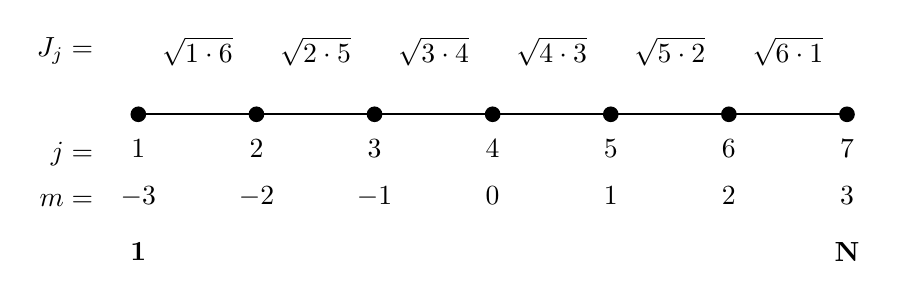
\begin{tikzpicture}[x=1.5cm,y=1cm]
        \tikzset{point/.style={circle, fill=black, inner sep=2pt}}
        % Main horizontal axis line
        \draw[thick] (0,0) -- (6,0);
        % index
        \node[anchor=east] at (-0.3, 0.8) {$J_j =$};
        \node[anchor=east] at (-0.3, -0.5) {$j =$};
        \node[anchor=east] at (-0.3, -1.1) {$m =$};
        % coupling str
        \node at (0.5, 0.8) {$\sqrt{1 \cdot 6}$};
        \node at (1.5, 0.8) {$\sqrt{2 \cdot 5}$};
        \node at (2.5, 0.8) {$\sqrt{3 \cdot 4}$};
        \node at (3.5, 0.8) {$\sqrt{4 \cdot 3}$};
        \node at (4.5, 0.8) {$\sqrt{5 \cdot 2}$};
        \node at (5.5, 0.8) {$\sqrt{6 \cdot 1}$};
        %  lattice dot
        \node[point] (N1) at (0,0) {};
        \node[point] (N2) at (1,0) {};
        \node[point] (N3) at (2,0) {};
        \node[point] (N4) at (3,0) {};
        \node[point] (N5) at (4,0) {};
        \node[point] (N6) at (5,0) {};
        \node[point] (N7) at (6,0) {};
        %  index n
        \node[anchor=north] at (0, -0.2) {$1$};
        \node[anchor=north] at (1, -0.2) {$2$};
        \node[anchor=north] at (2, -0.2) {$3$};
        \node[anchor=north] at (3, -0.2) {$4$};
        \node[anchor=north] at (4, -0.2) {$5$};
        \node[anchor=north] at (5, -0.2) {$6$};
        \node[anchor=north] at (6, -0.2) {$7$};
        % index m
        \node[anchor=north] at (0, -0.8) {$-3$};
        \node[anchor=north] at (1, -0.8) {$-2$};
        \node[anchor=north] at (2, -0.8) {$-1$};
        \node[anchor=north] at (3, -0.8) {$0$};
        \node[anchor=north] at (4, -0.8) {$1$};
        \node[anchor=north] at (5, -0.8) {$2$};
        \node[anchor=north] at (6, -0.8) {$3$};
        % site
        \node[anchor=north] at (0, -1.5) {$\mathbf{\ket{1}}$};
        \node[anchor=north] at (6, -1.5) {$\mathbf{\ket{N}}$};
    \end{tikzpicture}
    \caption*{Figure: Engineered coupling}
\end{figure}
This method offer PST in relatively short time, however it requires fine-tuning coupling strength for each spin interaction.
Hence, we want to avoid this for long $N$ case.
We begin by associating a fictitious spin $S = (N-1)/2$ particle with the chain and relabel the basis vectors as $\ket{m}$, where
\begin{equation*}
    m = -(N-1)/2+j-1 = -S +j -1
\end{equation*}
The input site can be labeled as $\mathbf{\ket{1}}  \to \ket{-(N-1)/2}$ and the output as $\ket{\mathbf{N}} \to \ket{+(N-1)/2}$.
Then we set magnetic field in such way that the diagonal vanishes, or equivalently we can start from XX Hamiltonian from the beginning.
What we are doing here is mapping our restricted $N$-dimensional one excitation sector to onto the Hilbert space of a fictitious single spin $S = (N-1)/2$.
Now recall the raising and lowering of spin operator
\begin{equation*}
    S_{\pm}   \ket{S, m} =  \sqrt{S(S+1) - m(m \pm 1)}   \ket{S, m \pm 1}
\end{equation*}
or by substituting the mapping $2S = N-1$ and $m +1  = j-S$
\begin{gather*}
    S_{+}   \ket{S, m} =  \frac{1 }{2 }\sqrt{j(N \mp j)}   \ket{S, m +  1}\\
    S_{-}   \ket{S, m} =  \frac{1 }{2 }\sqrt{(j-1(N-j+1))}   \ket{S, m - 1}
\end{gather*}
With this, we can determine the matrix element of $x$ component $S_x = (S_++S_-)/2$ as
\begin{equation*}
    \braket{j+1 | S_x|j} = \frac{1 }{2 }\sqrt{j(N-j)}
\end{equation*}
This is the same as the element of XX Hamiltonian up to scaling constant
\begin{equation*}
    \braket{j+1 | H|j} = \lambda J_j
\end{equation*}
after we use the coupling constraints
\begin{equation*}
    J_j = \sqrt{j(N-j)}
\end{equation*}
In any case, we have the matrix element
\begin{equation*}
    H  = -\lambda\begin{bmatrix}
        0      & J_{1}  & 0      & \cdots \\
        J_1    & 0      & J_2    & \cdots \\
        0      & J_2    & 0      & \cdots \\
        \vdots & \vdots & \vdots & \ddots
    \end{bmatrix}
\end{equation*}

Next we can write the propagator as
\begin{equation*}
    U(t) = \exp (-i \lambda t S_x)
\end{equation*}
which responsible for internal spin rotation.
The transfer amplitude $f_N = \braket{N |U(t)|1 }$ now reads after relabeling as
\begin{equation*}
    f_N = \braket{S,S |U(t) |S,-S} =D^{(S)}_{S,-S}
\end{equation*}
where $D^{(S)}_{S,-S} $ is the Wigner functions.
Here it represents amplitude for the rotated state to be found in $\ket{S,S}$ when the original unrotated state is given by $\ket{S,-S}$.
This element may be evaluated as
\begin{equation*}
    f_N= \left[-i\sin\left(\frac{\lambda t}{2}\right)\right]^{N_-1}
\end{equation*}
From this, it also can be seen that the fidelity reaches maximum at $t  = \pi/\lambda$.
The time it took for fidelity to reaches maximum is invariant of the $N$ because the dependence is already embedded at the coupling $J_j$ which scale $O(N)$ with $N$.
Compare to the coupling
\begin{equation*}
    J_j = \frac{2J }{N} \sqrt{j(N-j)}
\end{equation*}
which scale $O(1)$ with $N$.
Using this coupling, the optimum time scale with $N$, that is
\begin{equation*}
    t = \left[\frac{\pi}{4G_N}\alpha^2 + \frac{\pi}{6}(1-\alpha^2)\right]N
\end{equation*}
with $\alpha=1$ at PST.

\subsection{Localized eigenstates}
\begin{figure}
    \centering
    \begin{tikzpicture}[x=1.3cm,y=1cm]
        \tikzset{point/.style={circle, fill=black, inner sep=2pt}}
        \usetikzlibrary{decorations.pathmorphing}
        \draw[] (0,0) -- (3,0);
        \draw[] (3,0) -- (3.5,0);
        \draw[dotted] (3.5,0) -- (4.5,0);
        \draw[]  (4.5,0) -- (5,0);
        \draw[] (5,0) -- (8,0);

        % coupling strength
        \node at (0.5, 0.5) {$\alpha J_1$};
        \node at (1.5, 0.5) {$J_1$};
        \node at (2.5, 0.5) {$J_1$};
        \node at (5.5, 0.5) {$J_1$};
        \node at (6.5, 0.5) {$J_1$};
        \node at (7.5, 0.5) {$\alpha J_1$};
        \node at (1, 1.7) {$\alpha J_2$};
        \node at (2, 1.7) {$J_2$};
        \node at (6, 1.7) {$J_2$};
        \node at (7, 1.7) {$\alpha J_2$};


        \node[circle,fill=white] at (0,0) {};
        \draw[thick,->,>=Stealth] (0,-0.25) -- (0,0.25);
        \foreach \x in {1,2,3,5,6,7,8}{
                \node[circle,fill=white] at (\x,0) {};
                \draw[thick,->,>=Stealth] (\x,0.25) -- (\x,-0.25);
            }


        \node[anchor=north] at (0, -0.4) {$1$};
        \node[anchor=north] at (1, -0.4) {$2$};
        \node[anchor=north] at (2, -0.4) {$3$};
        \node[anchor=north] at (6, -0.4) {$N-2$};
        \node[anchor=north] at (7, -0.4) {$N-1$};
        \node[anchor=north] at (8, -0.4) {$N$};

        \draw[dash pattern=on 6pt off 1pt] (0,0.6) .. controls (0,1.4) and (2,1.4) .. (2,0.6);
        \draw[dash pattern=on 6pt off 1pt] (1,0.6) .. controls (1,1.4) and (3,1.4) .. (3,0.6);
        \draw[dash pattern=on 6pt off 1pt] (5,0.6) .. controls (5,1.4) and (7,1.4) .. (7,0.6);
        \draw[dash pattern=on 6pt off 1pt] (6,0.6) .. controls (6,1.4) and (8,1.4) .. (8,0.6);
    \end{tikzpicture}
    \caption*{Figure: Localized eigenstates realization via dangling coupling.}
\end{figure}

We start by considering the transition amplitude
\begin{equation*}
    f(t) = \sum_{j=1}^{N} e^{-i E_j t}\braket{\mathbf{r}|\tilde{m}_j }\braket{\tilde{m}_j |\mathbf{s} }
\end{equation*}
Defining the projection of eigenstates $\ket{\tilde{m}_j}$ to sender as $|\sigma_j| e ^{\phi_j}$ and to receiver as $|\rho_j| e ^{\psi_j}$, we have
\begin{equation*}
    f(t) = \sum_{j=1}^{N} e^{-i E_j t}\rho_j \sigma_j ^*
\end{equation*}
Then
\begin{align*}
    |f(t)|^2
     & = \left(\sum_j e^{-iE_j t}\rho_j\sigma_j^*\right)\left(\sum_l e^{iE_l t}\rho_l^*\sigma_l\right)
    =  \sum_{j,l} e^{-i(E_j-E_l)t}\rho_j\rho_l^*\sigma_j^*\sigma_l                                             \\
     & = \sum_{j,l}|\rho_j||\rho_l||\sigma_j||\sigma_l|e^{-i(E_j-E_l)t} e^{i[(\psi_j-\psi_l)-(\phi_j-\phi_l)]} \\
     & = \sum_{j=1}^N |\sigma_j|^2 |\rho_j|^2 + 2\sum_{k<l} |\sigma_k||\sigma_l||\rho_k||\rho_l|               \\
     & \qquad\times\cos\big([(E_l-E_k)t + (\psi_k-\psi_l) - (\phi_k-\phi_l)]\big) = f_m + f_t
\end{align*}
Since $|f(t)|^2\in [0,1]$ and $f_t$ oscillates rapidly, the allowed minimum value for $f_t$ is $-f_m$.
This implies that $2f_m$ is an accurate estimate for the maximum value of $|f(t)|^2$.
Hence, we investigate when
\begin{equation*}
    f_m = \sum_{j=1}^N |\sigma_j|^2 |\rho_j|^2
\end{equation*}
reaches its maximum value.
This search is bounded by the few normalization constraints.
First we write
\begin{align*}
    \braket{\mathbf{s} | \mathbf{s}}
     & =  \sum_{j } \braket{\mathbf{s }  | \tilde{m}_j } \braket{\tilde{m}_j  | \mathbf{s}}
    = \sum_{j } |\sigma_j|^2 = 1                                                            \\
    \braket{\mathbf{r} | \mathbf{r}}
     & =  \sum_{j } \braket{\mathbf{r }  | \tilde{m}_j } \braket{\tilde{m}_j  | \mathbf{r}}
    = \sum_{j } |\rho_j|^2 = 1
\end{align*}
For fixed $j$, we can also expand in terms of other one-excitation state
\begin{equation*}
    \braket{\tilde{m}_j  | \tilde{m}_j }
    = \sum_{ \mathbf{i} }  \braket{\tilde{m}_j  | \mathbf{i } } \braket{\mathbf{i }  | \tilde{m}_j }
    = \sum_{\mathbf{i} \neq (\mathbf{s},\mathbf{r})}  |\braket{\tilde{m}_j  | \mathbf{i }}|^2 + |\sigma_j|^2 + |\rho_j|^2 = 1
\end{equation*}
With the sum interior overlap as $|\gamma_j|^2$ (first term), we can write for fixed $j$
\begin{align*}
    |\sigma_j|^2|\rho_j|^2 = |\sigma_j|^2 \left( 1 - |\sigma_j|^2 -  |\gamma_j|^2\right)
    = \left( 1 - |\rho_j|^2 -  |\gamma_j|^2\right) |\rho_j|^2
\end{align*}
Setting the derivative with respect to $|\sigma_j|^2$ to zero
\begin{align*}
    \frac{d }{d|\sigma_j|^2} |\sigma_j|^2|\rho_j|^2 & =  1 - 2|\sigma_j|^2 -|\gamma_j|^2 = 0 \\
    \frac{d }{d|\rho_j|^2} |\sigma_j|^2|\rho_j|^2   & =  1 - 2|\rho_j|^2 -|\gamma_j|^2 = 0
\end{align*}
we find that
\begin{equation*}
    |\rho_j|^2 = |\sigma_j|^2 = \frac{1 - |\gamma_j |^2}{2}
\end{equation*}
Suppose that the eigenstate is entirely localized in the boundary, which imply $|\gamma_j|^2=0$, we have then
\begin{equation*}
    |\rho_j|^2 = |\sigma_j|^2 = \frac{1 }{2 }
\end{equation*}
Explicitly, our eigenstates is in the form
\begin{equation*}
    \ket{\tilde{m}_\pm} = \frac{1 }{\sqrt{2}} \left( \ket{\mathbf{s }} \pm \ket{\mathbf{r}} \right)
\end{equation*}
In this case, we have unitary amplitude
\begin{align*}
    f(t) & =
    e ^{-i E_+ t} \braket{\mathbf{r } |\tilde{m}_+ } \braket{\tilde{m}_+  | \mathbf{s}} +
    e ^{-i E_- t} \braket{\mathbf{r } |\tilde{m}_- } \braket{\tilde{m}_-  | \mathbf{s}}                                                              \\
         & = \frac{1 }{2 }e ^{-i E_+ t} - \frac{1 }{2} e ^{-i E_- t} = \frac{1}{2} e^{-i \bar{E} t}\left(e^{-i\Delta E t/2}-e^{i\Delta E t/2}\right) \\
         & = - i e ^{-i \bar{E} t}\sin \left( \Delta E t /2 \right)
\end{align*}
with $\bar{E} = (E_++E_-)/2$ and $\Delta E = E_+ - E_-$.
Hence, the fidelity
\begin{equation*}
    F(t) = \frac{1 }{6 } \sin^2 \left( \Delta E t /2 \right) + \frac{1 }{3 }\sin \left( \Delta E t /2 \right) + \frac{1 }{2 }
\end{equation*}
will reach maximum value at $t_m = \pi/\Delta E$.
Dual hole method is then applied by setting the coupling constants $J_{2,i}$ and $J_{N-1,i}$ to zero.
Sender and receiver are still found at the two ends of the chain, but now their nearest neighboring sites are empty.

We move to evaluating the eigenvalue using the discrete version $\textstyle\sum_{j} H_{ij}a_j^{\pm} = E_\pm a_i^{(\pm)}$.
For eigenstate localized at either end, we have $a^\pm_i=0$ for all $i$ except the boundary, and the effective eigenvalue equation is
\begin{equation*}
    \begin{bmatrix}
        H_{11} & H_{1N} \\
        H_{N1} & H_{NN}
    \end{bmatrix}
    \begin{bmatrix}
        a_1 \\
        a_N
    \end{bmatrix}
    =
    E
    \begin{bmatrix}
        a_1 \\
        a_N
    \end{bmatrix}
\end{equation*}
From the entire Hamiltonian space, this effective equation is obtained by projecting into $\mathrm{span} \{\ket{m_+},\ket{m_-}\}$.
Produce the characteristic equation
\begin{align*}
    (H_{11}-E)(H_{NN}-E)-H_{1N}H_{N1}                           & =  0 \\
    E^2-(H_{11}+H_{NN})E+\left(H_{11}H_{NN}-H_{1N}H_{N1}\right) & =  0
\end{align*}
Solving the quadratic equation
\begin{equation*}
    E_\pm=
    \frac{H_{11}+H_{NN}}{2}\pm\sqrt{\left(\frac{H_{11}-H_{NN}}{2}\right)^2+|H_{1N}|^2}
\end{equation*}
Both in XX and XXX case, the diagonal is the same, hence
\begin{equation*}
    E_\pm = H_{11} \pm |H_{1N}|\qquad
    \Delta E = 2|H_{1N}|
\end{equation*}
With $J_{1N} = 1/(2|N-1|^\nu)$, this reproduces $t_m = \pi(N-1)^\nu/2$.

\subsection{Localized Eigenstates for XX Hamiltonian}
XX Hamiltonian is known to be generally better at state transfer.
In particular, we choose the Hamiltonian
\begin{equation*}
    H =   -\sum_{r=1}^{N-1}J_r \sum_{i=1}^{N-r}  (\sigma_{z} ^{i} \sigma_z ^{i+r} + \sigma_{y} ^{i} \sigma_y ^{i+r})
    - \sum_{i } ^N B \sigma_{z}^i
\end{equation*}
where we considered also long-range effect $J_{ij} = C /(a|i-j|)^\nu$.
Here the magnetic field shall function for qubit energy splitting, so that its ergotropy exist.
In can be thought as merely energy shift in state transfer case.

Introducing imperfection $\alpha$ can create localized eigenstate which generally make better transport channel.
The Hamiltonian can be modified as
\begin{equation*}
    H= -\sum_{r=1}^{N-1}J_r \sum_{i=1}^{N-r} g_{i,r}(\alpha) \left( \sigma_x^i\sigma_x^{i+r} + \sigma_y^i\sigma_y^{i+r} \right) -B\sum_{i=1}^{N}\sigma_z^i
\end{equation*}
with the imperfection
\begin{equation*}
    g_{i,r}(\alpha)= \begin{cases} \alpha, & r=1 \ \text{and}\ \left(i=1\ \text{or}\ i+r=N\right), \\[2mm] 1, &\text{otherwise}. \end{cases}
\end{equation*}
and matrix representation
\begin{equation*}
    H_{ij}(\alpha)=
    \begin{cases}
        -2Jg_{ij}(\alpha), & i \neq j \\
        0,                 & i=j
    \end{cases}
\end{equation*}

The eigenvalue spectrum remain $E_k = -2J \cos k$, however the allowed $k $ must satisfy the transcendental equation below
\begin{equation*}
    \eta\cot k \left[ \cot\left(\frac{N-1}{2}k\right) \right]^\eta  = \frac{\alpha^2}{2-\alpha^2}
\end{equation*}
with parity $\eta=\pm1$.
The eigenvalue nearest to $E_0$ is given by 
\begin{equation*}
    \epsilon = \begin{cases} \dfrac{4J\alpha^2}{2-\alpha^2}\simeq2J\alpha^2, & N\; \mathrm{even},\\\\
         4J\sqrt{\dfrac{2\alpha^2}{(N-1)(2-\alpha^2)}}\simeq \frac{2 \sqrt{2}J\alpha }{\sqrt{N-1}}, & N\ \mathrm{odd}
         \end{cases}
\end{equation*}
The ratio $\epsilon_\text{odd}/\epsilon_\text{even}\simeq1/\alpha$ increase for small value of $\alpha \ll1$, hence under timescale $\tau\sim1/\epsilon$ odd $N$ evolves on a shorter thus resulting in better fidelity.
We can evaluate the optimum $\alpha$ under time constrain $(0,T)$ from this expression
\begin{equation*}
    \alpha_{\rm opt}=
    \begin{cases}
 \sqrt{\frac{2\pi}{8JT+\pi}} &\text{even }N\\\\
 \sqrt{ \frac{2\pi^2(N-1)} {32J^2T^2+\pi^2(N-1)} },&\text{odd }N
    \end{cases}
\end{equation*} 
Substituting $\alpha_\text{opt}$ back into $\epsilon$ yields the maximum transfer time again as expected, that is $t = \pi/2\epsilon$ for even $N$ and $t=\pi/\epsilon$ for odd $N$.

The eigenvector component $\braket{\mathbf{j} |m }$ reads similarly in boundary
\begin{equation*}
    a_1=\frac{\alpha}{c}\sin k \qquad
    a_N=\eta a_1 =\frac{\eta\alpha}{c}\sin k
\end{equation*}
While the bulk
\begin{equation*}
    a_i= \frac{1}{c} \left[ \sin(ik) + (1-\alpha^2)\sin((i-2)k) \right]
\end{equation*}
Here the normalization factor becomes
\begin{equation*}
    c^2 = (N-1) \left[ 2(1-\alpha^2)\cos^2k+\frac{\alpha^4}{2} \right] +2\alpha^2-\alpha^4
\end{equation*}

For long-range interaction, the Hamiltonian action on one-excitation state is
\begin{equation*}
    H\ket{\mathbf j}
    =
    -2\sum_{i\neq j}J_{ij}\ket{\mathbf i}
    -2B\ket{\mathbf j}
\end{equation*}
and the representation reads
\begin{equation*}
    H_{ij} =
    \begin{cases}
        H_{ij} =- 2J_{ij} & i\neq j \\\\
        H_{ii} = -2B      & i=j
    \end{cases}
\end{equation*}
This comes easily from
\begin{gather*}
    \sigma_i^x\sigma_j^x+\sigma_i^y\sigma_j^y=
    2P_{ij}-I-\sigma_i^z\sigma_j^z\\
    H_{XXX} \ket{\mathbf{j} } =
    -2\sum_{i \neq j}J_{ij}  \ket{\mathbf{i}} +2 \sum_{i \neq j}  J_{ij}\ket{\mathbf{j}} -2B\ket{\mathbf{j}}    \\
    \sum_{i<j} J_{ij} \sigma^z_i \sigma^z_j \ket{\mathbf{k}}
    = - 2 \sum_{i \neq k} J_{ik} \ket{\mathbf{k}}  + \sum_{i<j} J_{ij} \ket{\mathbf{k}}\\
    E_0 = -\sum_{i<j}J_{ij}
\end{gather*}
which I derived in long-range section of XXX Hamiltonian.
Also note that we use the shifted energy, hence all you do to obtain the result is to obey the first equation and add the final $E_0$.

\subsubsection{Odd and even chain length performance.}
For even \(N\), there is no symmetry-enforced zero mode.
Suppose that the dynamics is dominated by the two central states.
\begin{equation*}
    \ket{\psi_\pm} = \frac{\ket{\mathbf{1 }\pm \ket{\mathbf{N } } } }{\sqrt{2}}
\end{equation*}
with eigenvalue $\pm \epsilon$ respectively.
Their contribution to the transfer amplitude is
\begin{equation*}
    f_{N}(t)
    \simeq
    \sum_{\pm}
    e^{-iE_\pm t}
    \langle\mathbf N|\psi_\pm\rangle
    \langle\psi_\pm|\mathbf1\rangle .
\end{equation*}
In the idealized limit in which the two states have the endpoint form above, this reduces, up to a convention-dependent phase, to
\begin{align*}
    f_{N}(t) & \simeq
    \frac12
    \left(e^{-i\epsilon t}-e^{i\epsilon t}\right) \\
             & =
    \frac{1}{2}
    \left[
        \cos(\epsilon t)-i\sin(\epsilon t)
        -
        \cos(\epsilon t)-i\sin(\epsilon t)
    \right]                                       \\
             & =
    -i\sin(\epsilon t)
\end{align*}
which reaches maximum at $t=\pi/2\epsilon$
Hence, perfect transfer is obtained when the two central eigenstates acquire the appropriate relative phase, while their endpoint weights approach the limiting value (1/2).

\begin{figure}
    \centering
    \fullfig{../../../Rss/QM/Research_PST/eigenstate_oddeven.pdf}
    \caption*{Figure: Eigenstate population for odd $N=99$ and even $N=100$. For even $N$, the population is dominated by two central eigenstates, corresponding to the symmetric and antisymmetric combinations of the endpoint states. For odd $N$, three central eigenstates dominate: the zero-energy state $E_0$ and the two states with energies $\pm\epsilon$.}
\end{figure}

The structure of odd \(N\)  enforces an exact zero-energy eigenstate, which contribute greatly to the transfer.
Suppose that the dynamics is dominated by the three central states.
In the small-$\alpha$ limit, these states can be written as
\begin{equation*}
    \ket{\psi_0}
    \simeq
    \frac{\ket{\mathbf{1}}-\ket{\mathbf{N}}}{\sqrt{2}},
    \qquad
    E_0=0,
\end{equation*}
and
\begin{equation*}
    \ket{\psi_\pm}
    \simeq
    - \frac{1}{2}
    \left(
    \ket{\mathbf{1}}
    +
    \ket{\mathbf{N}}
    \right)
    + \ket{\phi_\pm},
    \qquad
    E_\pm=\pm\epsilon,
\end{equation*}
where $\ket{\phi_\pm}$ denotes the bulk component required for normalization.
Consequently,
\begin{align*}
    f_{N}(t)
     & \simeq
    \sum_{m=0,\pm}
    e^{-iE_m t}
    \langle\mathbf N|\psi_m\rangle
    \langle\psi_m|\mathbf1\rangle \\
    f_{N}(t)
     & \simeq
    \frac{1}{2}
    -
    \frac{1}{4}e^{-i\epsilon t}
    -
    \frac{1}{4}e^{i\epsilon t}    \\
     & =
    \frac{1}{2}
    -
    \frac{1}{4}
    \left[
        \cos(\epsilon t)-i\sin(\epsilon t)
        \right]
    -
    \frac{1}{4}
    \left[
        \cos(\epsilon t)+i\sin(\epsilon t)
    \right]                       \\
     & =
    \frac{1}{2}
    -
    \frac{1}{2}\cos(\epsilon t)   \\
     & =
    \sin^2\left(\frac{\epsilon t}{2}\right).
\end{align*}
which reach maximum at $t = \pi/\epsilon$.
We observe that the odd N guarantee $E_0$ eigenstate with weight of $(1/2)$ such that the remaining eigenstates only $(1/2)$, hence the localization requirement is less stringent in this case.
We observe that for odd \(N\), the spectrum necessarily contains a zero-energy eigenstate \(E_0=0\).


\begin{figure}
    \centering
    \fullfig{../../../Rss/QM/Research_PST/Ergo_compare_oddeven.pdf}
    \caption*{Figure: Optimal $\alpha$ for odd $N=99$ (blue curve) and even $N=100$ (red curve). The even-$N$ chain exhibits greater sensitivity to variations in $\alpha$, indicating a narrower range of $\alpha$ values that yields high transfer fidelity.}
\end{figure}

For even \(N\), the two central states must do essentially all the endpoint transfer.
Therefore, their localization must be relatively strong before the two-state approximation works well.
For odd \(N\), the zero mode already supplies approximately $1/2$ to the transfer amplitude.
Since it accounts for half of the endpoint spectral weight, the non-zero eigenstates only the remaining $1/2$.
Thus, the odd chain can retain good transfer even when \(\epsilon_\pm\) eigenstates are not as strongly localized.
This means that, the odd chain can tolerate a broader range of \(\alpha\) while retaining substantial transfer.
This is consistent with our observation where the optimal coupling for an odd $N$ is applied to an even chain, the transfer fidelity is strongly suppressed; whereas applying the optimal coupling for an even $N$ to an odd chain results in a comparatively smaller reduction in fidelity.


We observe that odd-\(N\) chains exhibit a larger energy splitting than even-\(N\) chains, resulting in a shorter characteristic transfer timescale.
Consequently, the odd-\(N\) chains can achieve high-fidelity state transfer within the finite evolution window \(0<t<1000\), leading to improved transfer performance compared with even-\(N\) chains.

\begin{figure}
    \centering
    \fullfig{../../../Rss/QM/Research_PST/epsilon_vs_alp.pdf}
    \caption*{Figure: Energy splitting each $N$ using optimum $\alpha$. Black curve and diamond marker denote numeric and analytic result.}
\end{figure}

This argument rest on the fact that odd $N$ guarantee ground state exist, and that the eigenstate associated is completely localized.
This can be proved as follows.
In the one-excitation subspace, the nearest-neighbor XX Hamiltonian has the form
\begin{equation*}
    H =
    -2J
    \begin{pmatrix}
        0      & \alpha & 0      & \cdots & 0      \\
        \alpha & 0      & 1      & \cdots & 0      \\
        0      & 1      & 0      & \ddots & \vdots \\
        \vdots & \vdots & \ddots & \ddots & \alpha \\
        0      & 0      & \cdots & \alpha & 0
    \end{pmatrix}
    = \begin{pmatrix} 0 & c_1 & 0 & \cdots & 0 \\ b_1 & 0 & c_2 & \cdots & 0 \\ 0 & b_2 & 0 & \ddots & \vdots \\ \vdots & \vdots & \ddots & \ddots & c_{N-1} \\ 0 & 0 & \cdots & b_{N-1} & 0 \end{pmatrix}
\end{equation*}
The determinant satisfies the standard tridiagonal recurrence relation
\begin{align*}
    \det(A_k) & =  d_k \det(A_{k-1}) - b_{k-1}c_{k-1} \det(A_{k-2}) \\
    \det(A_k) & = -b_{k-1}c_{k-1} \det(A_{k-2})
\end{align*}
where $d_k$ is the $k$-th entry on the main diagonal.
Starting with the base conditions of $k = 1$ we have $\det(A_1) = |0| = 0$, so that for every odd integer $N$,
\begin{equation*}
    \det(A_N) = 0
\end{equation*}
Recall that the eigenvalues of $H$ are the roots of its characteristic polynomial
\begin{equation*}
    p(\lambda) = \det(A - \lambda I) = 0
\end{equation*}
It can be seen that $\det A = 0$ prove that $\lambda=0$ is one of the root
\begin{equation*}
    p(0) = \det(A - 0\cdot I) = \det A = 0
\end{equation*}
Hence odd $N$ does have $E_0$ eigenvalue.
The corresponding eigenstate can be obtained directly from the eigenvalue equations
\begin{equation*}
    E a_i=
    \begin{cases}
        -2J\alpha a_2,              & i=1,           \\
        -2J(\alpha a_{1}+a_{3}),    & i = 2,         \\
        -2J(a_{i-1}+a_{i+1}),       & 3\le i\le N-2, \\
        -2J( a_{N-2}+\alpha a_{N}), & i = N-1,       \\
        -2J\alpha a_{N-1},          & i=N.
    \end{cases}
\end{equation*}
For $\alpha\neq0$, $i=1$ and $i=N$ equations imply
\begin{equation*}
    a_2=a_{N-1}=0.
\end{equation*}
The bulk recurrence relation then gives
\begin{equation*}
    a_{i+2}=-a_{i}.
\end{equation*}
Writing $N=2M+1$, we see all even-site amplitudes vanish,
\begin{equation*}
    a_{2m}=0,
\end{equation*}
whereas the odd-site $3,\dots,N-2$ amplitudes satisfy
\begin{equation*}
    a_{2m+1}=(-1)^m\alpha a_1,
    \qquad
    1\leq m\leq M-1.
\end{equation*}
The right boundary condition yields
\begin{equation*}
    a_N=-\frac{a_{N-2}}{\alpha}
\end{equation*}
so, using the result for $m=M-1$
\begin{equation*}
    a_N = -(-1)^{M-1} a_1.=(-1)^M a_1.
\end{equation*}
Thus, up to normalization, the zero-energy eigenstate is
\begin{equation*}
    \ket{\psi_0}
    \propto
    \left[\ket{1}+(-1)^M\ket{N}+\alpha\sum_{m=1}^{M-1}(-1)^m\ket{2m+1}\right],
\end{equation*}
Normalization gives
\begin{equation*}
    \langle\psi_0|\psi_0\rangle = 1+1+ \alpha^2\sum_{m=1}^{M-1}1=2+\alpha^2(M-1)
\end{equation*}
as constant.
So accurately we write
\begin{equation*}
    \ket{\psi_0}
    =
    \frac{\ket{1}+(-1)^M\ket{N}+ \alpha \sum_{m=1}^{M-1}(-1)^m\ket{2m+1}}{\sqrt{2+\alpha^2(M-1)}}
\end{equation*}
Therefore,
\begin{equation*}
    \lim_{\alpha\rightarrow0^+}
    \ket{\psi_0}=
    \frac{
        \ket{1}+(-1)^M\ket{N}
    }{\sqrt{2}},
\end{equation*}
up to an overall phase. The zero-energy eigenstate is consequently localized entirely within the endpoint subspace in the weak-coupling limit.

\begin{figure}
    \centering
    \fullfig{../../../Rss/QM/Research_PST/alpvals_oddeven.pdf}
    \caption*{Figure: Numerical (red) and analytic (blue) optimal $\alpha$ for each spin length $N$.}
\end{figure}

\subsubsection{Derivation: dual hole coupling eigenvalue.}
Now suppose we introduce dual hole coupling, which turn the Hamiltonian into
\begin{equation*}
    H_{ij}(\alpha)=
    \begin{cases}
        -2Jg_{ij}(\alpha), & i \neq j \\
        0,                 & i=j
    \end{cases}
\end{equation*}
with
\begin{equation*}
    g_{ij}(\alpha)=
    \begin{cases}
        \alpha,
         & |i-j|=1
        \ \text{and}\
        \left(i\in\{1,N\}\ \text{or}\ j\in\{1,N\}\right),
        \\
        1,
         & |i-j|=1 \\
    \end{cases}
\end{equation*}
Aside, for long range coupling, we can modify $g(\alpha)$ into
\begin{equation*}
    g_{ij}(\alpha)=
    \begin{cases}
        \alpha,
         & i\in\{1,N\}\ \text{or}\ j\in\{1,N\} \\
        1,
         & \text{otherwise}                    \\
    \end{cases}
\end{equation*}
Of course, we change also the coupling itself into  site dependent one $J_{ij}$.
In any case, the discrete Hamiltonian  $\textstyle\sum_j H_{ij}a_j = E a_i$ reads
\begin{equation*}
    E a_i=
    \begin{cases}
        -2J\alpha a_2,              & i=1,           \\
        -2J(\alpha a_{1}+a_{3}),    & i = 2,         \\
        -2J(a_{i-1}+a_{i+1}),       & 3\le i\le N-2, \\
        -2J( a_{N-2}+\alpha a_{N}), & i = N-1,       \\
        -2J\alpha a_{N-1},          & i=N.
    \end{cases}
\end{equation*}
From the bulk case, we earlier obtain the general form of
\begin{equation*}
    a_j = Ae^{ikj} + B e^{-ikj} = A \sin (kj+\delta)
\end{equation*}
With $\lambda = -E/2J = 2 \cos k$, at $i=1$ we have
\begin{align*}
    \lambda a_1=\alpha a_2\implies a_1  = \alpha a_2/\lambda
\end{align*}
so that at $i=2$
\begin{align*}
    \lambda a_2                                 & = \alpha a_1+a_3                            \\
    \lambda a_2                                 & = \alpha(\alpha a_2/\lambda)+a_3            \\
    (\lambda^2-\alpha^2)a_2                     & = \lambda a_3                               \\
    a_2                                         & = \frac{\lambda}{\lambda^2-\alpha^2}a_3     \\
    \frac{\sin (2j+\delta )}{\sin (3j+\delta )} & = \frac{2\cos ^2 k}{4 \cos ^2k-\alpha^2}a_3
\end{align*}

Because the Hamiltonian is invariant under the reflection \(j\mapsto N+1-j\), its eigenstates can be chosen to have definite parity $a_{N+1-j}=\eta a_j$, with $\eta=\pm1$.
Using the bulk form, the reflection condition becomes
\begin{equation*}
    \sin\left[k(N+1-j)+\delta\right]=\eta\sin(kj+\delta)
\end{equation*}
In symmetric sector $\eta=+1$, the reflection reads
\begin{align*}
    \sin\left[k(N+1-j)+\delta\right] & = \sin(kj+\delta)            \\
    k(N+1-j)+\delta                  & = \pi-(kj+\delta)+2\pi n     \\
    k(N+1)+2\delta                   & = (2n+1)\pi                  \\
    \delta                           & = \frac{(2n+1)\pi-k(N+1)}{2}
\end{align*}
We have the arguments
\begin{equation*}
    \begin{cases}
        2k+\delta = \frac{(2n+1)\pi}{2} -\frac{N-3}{2}k
        \\
        3k+\delta = \frac{(2n+1)\pi}{2} -\frac{N-5}{2}k
    \end{cases}
\end{equation*}
Since
\begin{equation*}
    \sin\left(\frac{(2n+1)\pi}{2}-x\right) = (-1)^n\cos x
\end{equation*}
we have
\begin{equation*}
    \begin{cases}
        \sin(2k+\delta) = (-1)^n \cos\left(\frac{N-3}{2}k\right) \\
        \sin(3k+\delta) = (-1)^n \cos\left(\frac{N-5}{2}k\right)
    \end{cases}
\end{equation*}
Substituting to $i=2$ condition
\begin{align*}
    \frac{ \cos\left(\frac{N-3}{2}k\right)} { \cos\left(\frac{N-5}{2}k\right) }
           & = \frac{\cos A}{\cos(A-k)}
    =  \frac{2\cos k}{4\cos^2k-\alpha^2}                         \\
           & = \frac{1}{\cos k+\tan A\sin k}                     \\
    \tan A & =  \frac{4\cos^2k-\alpha^2-2\cos^2k}{2\cos k\sin k}
\end{align*}
then using
\begin{align*}
    \tan(A+k)                                & = \frac{\tan A+\tan k} {1-\tan A\tan k}                                                                                                           \\
                                             & = \frac{ \dfrac{2\cos^2k-\alpha^2}{2\sin k\cos k} +\dfrac{\sin k}{\cos k} }{ 1- \dfrac{2\cos^2k-\alpha^2}{2\sin k\cos k} \dfrac{\sin k}{\cos k} } \\
                                             & = \frac{2-\alpha^2}{2\sin k\cos k} \frac{2\cos^2k}{\alpha^2}                                                                                      \\
    \tan\left(\frac{N-1}{2}k\right)          & =  \frac{2-\alpha^2}{\alpha^2}\cot k                                                                                                              \\
    \tan k\, \tan\left(\frac{N-1}{2}k\right) & =  \frac{2-\alpha^2}{\alpha^2}                                                                                                                    \\
    \cot k\, \cot\left(\frac{N-1}{2}k\right) & =  \frac{\alpha^2}{2-\alpha^2}
\end{align*}

Next for the antisymmetric $\eta=-1$, our reflection reads
Now impose
\begin{align*}
    \sin\left[k(N+1-j)+\delta\right] & =  -\sin(kj+\delta)      \\
    k(N+1-j)+\delta                  & =  -(kj+\delta)+2\pi n   \\
    k(N+1)+2\delta                   & =  2\pi n                \\
    \delta                           & =  n\pi-\frac{k(N+1)}{2}
\end{align*}
Again, evaluate the two relevant arguments
\begin{equation*}
    \begin{cases}
        2k+\delta = n\pi-\frac{N-3}{2}k \\
        3k+\delta = n\pi-\frac{N-5}{2}k
    \end{cases}
\end{equation*}
and therefore
\begin{equation*}
    \begin{cases}
        \sin(2k+\delta) = (-1)^{n+1} \sin\left(\frac{N-3}{2}k\right) \\
        \sin(3k+\delta) = (-1)^{n+1} \sin\left(\frac{N-5}{2}k\right)
    \end{cases}
\end{equation*}
Then
\begin{align*}
    \frac{ \sin\left(\frac{N-5}{2}k\right) }{ \sin\left(\frac{N-3}{2}k\right)} & =  \frac{\sin(x-k)}{\sin(x)} = \frac{4\cos^2k-\alpha^2}{2\cos k} \\
    \cos k-\cot x\sin k                                                        & =  \frac{4\cos^2k-\alpha^2}{2\cos k}                             \\
    -\cot x\sin k                                                              & =  \frac{2\cos^2k-\alpha^2}{2\cos k}                             \\
    \tan x                                                                     & =  -\frac{2\sin k\cos k} {2\cos^2k-\alpha^2}
\end{align*}
Using the same identity
\begin{align*}
    \tan(x+k)                                 & =  \frac{\tan x+\tan k} {1-\tan x\tan k}                                                                                \\
                                              & =  \frac{ -\dfrac{2\sin k\cos k}{2\cos^2k-\alpha^2} +\dfrac{\sin k}{\cos k} }{ 1+ \dfrac{2\sin^2k}{2\cos^2k-\alpha^2} } \\
                                              & = \frac{\sin k}{\cos k} \frac{ -(2\cos^2k)+(2\cos^2k-\alpha^2) }{ 2\cos^2k-\alpha^2 }                                   \\
                                              & \qquad\bigg\slash\frac{ 2\cos^2k-\alpha^2+2\sin^2k }{ 2\cos^2k-\alpha^2 }                                               \\
                                              & =  -\frac{\alpha^2\sin k} {\cos k(2\cos^2k-\alpha^2)}\frac{2\cos^2k-\alpha^2}{2-\alpha^2}                               \\
    \tan\left(\frac{N-1}{2}k\right)
                                              & = -\frac{\alpha^2}{2-\alpha^2}\tan k                                                                                    \\
    -\cot k\, \tan\left(\frac{N-1}{2}k\right) & =  \frac{\alpha^2}{2-\alpha^2}.
\end{align*}
Combining both result based on symmetry
both equations become
\begin{equation*}
    \eta\cot k \left[ \cot\left(\frac{N-1}{2}k\right) \right]^\eta  = \frac{\alpha^2}{2-\alpha^2}
\end{equation*}

Now let's do sanity check on the transcendental equation.
For $\alpha=1$, the uniform coupling $k = m\pi/(N+1)$ should holds true.
Write the parity $\eta = (-1)^{m+1}$
\begin{align*}
    (-1)^{m+1}\cot k \left[ \cot\left(\frac{m\pi}{2}-k\right) \right]^{(-1)^{m+1}}
                                                             & = 1 \\
    s\cot k \left[ s\left\{ \tan k \right\}^{s}  \right]^{s} & = 1 \\
    s\cot (k) s^s \tan k                                     & = 1 \\
    s^{1+s}                                                  & = 1
\end{align*}
since $s=\eta = \pm1$, this is true.

\subsubsection{Derivation: Nearest ground state eigenvalue.}
\begin{table}
    \centering
    \begin{tabular}{cc}
        \toprule
        $N\bmod4$ & form        \\
        \midrule
        0         & $ N=4\ell$  \\
        1         & $N=4\ell+1$ \\
        2         & $N=4\ell+2$ \\
        3         & $N=4\ell+3$ \\
        \bottomrule
    \end{tabular}
\end{table}
With the eigenvalue $E = -4J \cos k$, the eigenvalue closest to $E_0$ correspond to $k = \pi/2$.
Then
\begin{equation*}
    E=-4J\cos\left(\frac{\pi}{2}+\delta\right) =4J\sin\delta \simeq 4J\delta
\end{equation*}
we need to determine $\delta$.
Consider the transcendental equation in this approximation
\begin{align*}
    \eta\cot \left(\frac{\pi}{2}+\delta\right) \left[ \cot\left(\frac{(N-1)\pi}{4} +\frac{N-1}{2}\delta\right) \right]^\eta
                                                                                                & =  \frac{\alpha^2}{2-\alpha^2}     \\
    -\eta\delta \left[ \cot\left( \frac{(N-1)\pi}{4} + \frac{N-1}{2}\delta \right) \right]^\eta & \simeq \frac{\alpha^2}{2-\alpha^2}
\end{align*}
Cotangent term behavior depend on \(N\bmod 4\); in particular, odd $N$ can be written as $4N\ell+1$ and $4N\ell+3$, while even $N$ as $4N\ell$ and $4N\ell+2$. 
For $N \bmod4 = 0$, we write $N=4\ell$ so that the cotangent argument reads 
\begin{equation*}
\frac{(4\ell-1)\pi}{4}+\frac{N-1}{2}\delta
=\ell\pi -\frac{\pi}{4}+\frac{N-1}{2}\delta
= -\frac{\pi}{4}+\frac{N-1}{2}\delta
\end{equation*}
Then for small $\delta\ll 2/(N-1)$, we can approximate
\begin{align*}
 -\eta\delta \left[-1\right]^\eta 
 &\simeq \frac{\alpha^2}{2-\alpha^2}\\
 \delta_{0}
 &\simeq \frac{\alpha^2}{\eta(-1)^\eta(\alpha^2-2)}
 =\frac{\eta\alpha^2}{(2-\alpha^2)}
\end{align*}
using $\cot x-\pi/4 = -1-2x+O(x^2)$.
To put it in other way, this approximation valid if $N\alpha^2\ll1$.

Now for $N\bmod4=1$ using $N=4\ell+1$,
\begin{equation*}
\frac{(4\ell)\pi}{4}+\frac{N-1}{2}\delta
=\ell\pi+\frac{N-1}{2}\delta
= \frac{N-1}{2}\delta
\end{equation*}
Approximating
\begin{align*}
-\eta\delta
\left[
\frac{2}{(N-1)\delta}
\right]^\eta
&\simeq \frac{\alpha^2}{2-\alpha^2}\\
\end{align*}
using $\cot x = 1/x+O(x)$. 
Now consider for $\eta=+1$, we have $\delta^{1-1}$ and the equation
Thus
\begin{equation*}
    -\frac{2}{N-1} = \frac{\alpha^2}{2-\alpha^2}
\end{equation*}
For the physical regime \(0<\alpha<1\), the right-hand side is positive, so this equation cannot be satisfied by this approximation around $k=\pi/2$.
For the other parity, we have 
\begin{align*}
    \delta_1^2 & =  \frac{2\alpha^2} {(N-1)(2-\alpha^2)}\\
    \delta_1 & =  \pm \sqrt{ \frac{2\alpha^2} {(N-1)(2-\alpha^2)} } 
\end{align*}

Next $N \bmod 4 =2$ using $N=4\ell+2$, we expect it produces the same behavior as $\delta_0$ since both denote even $N$.
\begin{equation*}
\frac{(4\ell+1)\pi}{4}+\frac{N-1}{2}\delta
=\ell\pi +\frac{\pi}{4}+\frac{N-1}{2}\delta
= -\frac{\pi}{4}+\frac{N-1}{2}\delta
\end{equation*}
Then for small $\delta\ll 2/(N-1)$, we can approximate
\begin{align*}
 -\eta\delta \left[-1\right]^\eta 
 &\simeq \frac{\alpha^2}{2-\alpha^2}\\
 \delta_{2}
 &\simeq \frac{\alpha^2}{\eta(\alpha^2-2)}
 =\frac{\eta\alpha^2}{(2-\alpha^2)}
\end{align*}
using $\cot x+\pi/4 = 1+2x+O(x^2)$ again.

In the same manner, we hope $N\bmod4=3$ using $N=4\ell+3$ produces the same result as $\delta_3$
\begin{equation*}
\frac{(4\ell+2)\pi}{4}+\frac{N-1}{2}\delta
=\ell\pi+ \frac{\pi}{2}+\frac{N-1}{2}\delta
= \frac{\pi}{2}+\frac{N-1}{2}\delta
\end{equation*}
Approximating
\begin{align*}
\eta\delta
\left[
\frac{(N-1)}{2}\delta
\right]^\eta
&\simeq \frac{\alpha^2}{2-\alpha^2}\\
\end{align*}
using $\cot x+\pi/2=-\tan x = -x+O(x^2)$. 
In this case, we throw the parity $\eta=-1$, which reads
\begin{equation*}
    -\frac{2}{N-1} = \frac{\alpha^2}{2-\alpha^2}
\end{equation*}
For the other parity, we have 
\begin{align*}
    \delta_3^2 & =  \frac{2\alpha^2} {(N-1)(2-\alpha^2)}\\
    \delta_3 & =  \pm \sqrt{ \frac{2\alpha^2} {(N-1)(2-\alpha^2)} } 
\end{align*}
This give the nearest eigenvalue
\begin{equation*}
    \epsilon = \begin{cases} \dfrac{4J\alpha^2}{2-\alpha^2}, & N\; \mathrm{even},\\\\
         4J\sqrt{\dfrac{2\alpha^2}{(N-1)(2-\alpha^2)}}, & N\ \mathrm{odd}
         \end{cases}
\end{equation*}

Now that the energy splitting expression is obtained, we can determine the optimum alpha under time constrain $(0,T)$.
For even $N$, the maximum time is $t=\pi/2\epsilon$, hence
\begin{align*}
T & =  \frac{\pi}{2} \frac{2-\alpha^2}{4J\alpha^2}\\
8JT\alpha^2 & = \pi(2-\alpha^2)\\
(8JT+\pi)\alpha^2 & = 2\pi\\
 \alpha_{\rm opt}^{\rm even}(T) & =  \sqrt{\frac{2\pi}{8JT+\pi}} 
\end{align*}
Whereas odd $N$ we have 
\begin{align*}
T&= \frac{\pi}{4J} \sqrt{ \frac{(N-1)(2-\alpha^2)} {2\alpha^2} }\\
\frac{16J^2T^2}{\pi^2} &= \frac{(N-1)(2-\alpha^2)} {2\alpha^2}\\
32J^2T^2\alpha^2 &= \pi^2(N-1)(2-\alpha^2)\\
\left[ 32J^2T^2+\pi^2(N-1) \right]\alpha^2 &= 2\pi^2(N-1)\\
 \alpha_{\rm opt}^{\rm odd}(N,T) &= \sqrt{ \frac{2\pi^2(N-1)} {32J^2T^2+\pi^2(N-1)} }
\end{align*}

\subsection{Arbitrary Qubit State}
\subsubsection{Coherrence and population state.}
Suppose we are given the pure and mixed state of spin chain in the form
\begin{gather*}
  \ket{\psi(0)} = \left(\alpha\ket{0}_1 + \beta\ket{1}_1\right)\bigotimes_{i=2}^{N}\ket{0}_i  = \alpha\ket{\mathbf{0}} + \beta\ket{\mathbf{1}}\\
  \rho(0) = \left(q\ket{1}\bra{1}_1 + (1-q)\ket{0}\bra{0}_1\right)\bigotimes_{i=2}^{N}\ket{0}\bra{0}_i = q\ket{\mathbf{1}}\bra{\mathbf{1}} + (1-q)\ket{\mathbf{0}}\bra{\mathbf{0}}
\end{gather*}
with $q = (1+|\beta^2|)/2$.
The first lines written in such way to demonstrate that the first site of spin chain is initially pure and mixed respectively.
Also, we do not simply set $q=|\beta|^2$ so that, with the same choice of $\alpha$ and $\beta$, the initial state of both pure state and mixed state encode the same initial ergotropy.
Alternatively, the state can be written as
\begin{equation*}
  \rho_\text{coh}
  = \begin{bmatrix}
    \alpha^2    & \alpha\beta^* \\
    \alpha\beta & |\beta|^2
  \end{bmatrix}
  \otimes \rho_\text{chain}
  \qquad
  \rho_\text{pop}
  = \begin{bmatrix}
    1-q & 0 \\
    0   & q
  \end{bmatrix}
  \otimes \rho_\text{chain}
\end{equation*}
As usual the pure state exist on the surface of Bloch sphere, while the mixed state on the interior, specifically on $z$ axis with $z = 1-2q$.

\begin{figure}
  \centering
  \begin{tikzpicture}[tdplot_main_coords,scale=3.5]
    \coordinate (O) at (0,0,0);
    \def\r{1}
    \def\th{50}
    \def\ph{70}
    \def\phm{-\ph}
    \pgfmathsetmacro{\rxy }{sin(\th)}

    \draw[thick,->] (O) -- (1.1,0,0) node[anchor=north east]{$\hat{x}$};
    \draw[thick,->] (O) -- (0,1.1,0) node[anchor=north west]{$\hat{y}$};
    \draw[thick,->] (O) -- (0,0,1.1) node[anchor=south]{$\hat{z}$};
    \shade[ball color=white, opacity=0.1] (0,0,0) circle (1);

    \tdplotsetcoord{A}{\r}{\th}{\ph}
    \tdplotsetcoord{Ath}{\r}{\th/2}{\ph}
    \tdplotsetcoord{A2}{\r}{\th}{\phm}
    \tdplotsetcoord{A2th}{\r}{\th/2}{\phm}
    \coordinate (P) at ({sin(\th)*cos(\ph)},0,{cos(\th)});

    \draw[dashed] (A) -- node[midway,midway,xshift=-15pt,yshift=-8pt, left] {$1-p$}  node[midway,xshift=20pt,yshift=-12pt, right] {$ p$} (A2) ;

    \tdplotdrawarc[->]{(O)}{0.2}{0}{\ph}{anchor=north}{$\phi$}
    \tdplotdrawarc[->]{(O)}{0.2}{0}{\phm}{anchor=north east}{$-\phi$}
    \tdplotsetthetaplanecoords{\ph}
    \tdplotdrawarc[->,tdplot_rotated_coords]{(O)}{0.2}{0}{\th}{anchor=south west
    }{$\theta$}
    \tdplotsetthetaplanecoords{\phm}
    \tdplotdrawarc[->,tdplot_rotated_coords]{(O)}{0.2}{0}{\th}{anchor=south east}{$\theta$}

    \draw[dashed]  (O) -- (Axy);
    \draw[dashed]  (A) -- (Axy);
    \draw[dashed]  (O) -- (A2xy);
    \draw[dashed]  (A2) -- (A2xy);

    \begin{scope}[tdplot_main_coords]
      \pgfmathsetmacro{\gamma}{acos(sin(\th)*sin(\th)*cos(\ph-\phm)+cos(\th)*cos(\th))}
      \draw[dashed,domain=0:1,samples=100,smooth]
      plot (
      {sin((1-\x)*\gamma)/sin(\gamma)*sin(\th)*cos(\ph)+sin(\x*\gamma)/sin(\gamma)*sin(\th)*cos(\phm)},
      {sin((1-\x)*\gamma)/sin(\gamma)*sin(\th)*sin(\ph)+sin(\x*\gamma)/sin(\gamma)*sin(\th)*sin(\phm)},
      {cos(\th)}
      );
      \draw[dashed,domain=0:1,samples=100,smooth]
      plot (
      {{sin(\th)*cos(\ph)}},
      {sin((1-\x)*\gamma)/sin(\gamma)*sin(\th)*sin(\ph)+sin(\x*\gamma)/sin(\gamma)*sin(\th)*sin(\phm)},
      {sin((1-\x)*\gamma)/sin(\gamma)*cos(\th)+sin(\x*\gamma)/sin(\gamma)*cos(\th)}
      );
    \end{scope}

    \node[circle,fill=white] at (A) {};
    \node[circle,fill=white] at (A2) {};
    \node[circle,fill=white] at (P) {};
    \draw[thick,->,>=Stealth] (O) -- (A) node [anchor=south west]{$\ket{\psi_1}$};
    \draw[thick,->,>=Stealth] (O) -- (A2) node [anchor=south east]{$\ket{\psi_2}$};
    \draw[thick,->,>=Stealth] (O) -- (P) node [anchor=south ]{$\rho$};

    \def\alp{20}
    \def\bet{70}
    \tdplotsetrotatedcoords{\alp}{0}{0}
    \begin{scope}[tdplot_rotated_coords]
      \draw[thick] (0,-\r) arc (-90:90:\r);
      \draw[dashed] (0,\r) arc (90:270:\r);
    \end{scope}

    \tdplotsetrotatedcoords{\alp}{\bet}{0}
    \begin{scope}[tdplot_rotated_coords]
      \draw[thick] (0,\r) arc (90:270:\r);
      % \draw[thick] (\r,0) arc (0:360:\r);
    \end{scope}
  \end{tikzpicture}
  \caption*{Figure: Bloch sphere representation of mixed states created from pure state $\ket{\psi_i}$ ensemble in $C_3$.}
  \label{fig:chain}
\end{figure}

\subsubsection{Pure state ensemble.}
Now suppose we create an ensemble the pure state
\begin{equation*}
  \ket{\psi_i}
  =
  \cos\frac{\theta_i}{2}\ket{0}
  +
  e^{i\phi_i}\sin\frac{\theta_i}{2}\ket{1},
\end{equation*}
The expression for this state is
\begin{equation*}
  \rho^{(1)}  =
  \begin{bmatrix}
    p\cos^2\frac{\theta_i}{2}
    +(1-p)\cos^2\frac{\theta_j}{2}
     &
    p e^{-i\phi_i}\frac{\sin \theta_i}{2}
    +(1-p)e^{-i\phi_j}\frac{\sin \theta_j}{2}
    \\\\
    p e^{i\phi_i}\frac{\sin \theta_i}{2}
    +(1-p)e^{i\phi_j}\frac{\sin \theta_j}{2}
     &
    p\sin^2\frac{\theta_i}{2}
    +(1-p)\sin^2\frac{\theta_j}{2}
  \end{bmatrix}
\end{equation*}
To simplify our expression, we can use the following parametrization: \((\theta_j,\phi_j)=(-\theta_i,-\phi_i)\), \((\theta_i,-\phi_i)\), and \((-\theta_i,\phi_i)\); respectively we define these constraints as $C_2$, $C_3$, and $C_4$.
The constraints are sufficient to parameterize the complete single-qubit state space.
By varying the parameters $(\theta,\phi,p)$, every physical qubit state within and on the surface of the Bloch sphere can be represented under each constraint.
Note that negative \(\theta\) should be interpreted as a parametrization device, rather than as a conventional polar angle, since $0 \leq \theta \leq \pi$.
Equivalently, the negative $\theta$ constraint can be represented by $(\theta_2=\theta_1,\phi_2 = \pi-\phi_1)$ and $(\theta_2=\theta_1,\phi_2 = \pi+\phi_1)$.


To avoid misinterpretation, we therefore choose the third constrain \((\theta_1,-\phi_1)\).
The state in this case is given by
\begin{equation*}
  \rho ^{(1)} =
  \begin{bmatrix}
    \cos ^2 \theta/2                                                 & \frac{\sin \theta}{2} \left[-i2p \sin \phi + e^{i\phi}  \right] \\
    \frac{\sin \theta  }{2} \left[i2p \sin\phi + e^{-i\phi}  \right] & \sin ^2 \frac{\theta  }{2}
  \end{bmatrix}
\end{equation*}
The last site then will carry the information from the first state and evolve as
\begin{equation*}
  \rho ^{(N)}  =
  \begin{bmatrix}
    1- \sin^2 \theta/2 |f_N|^2                                             & \frac{\sin \theta}{2} \left[-i2p \sin \phi + e^{i\phi}  \right]f_N \\
    \frac{\sin \theta  }{2} \left[i2p \sin\phi + e^{-i\phi}  \right]f_N ^* & \sin ^2 \frac{\theta  }{2}|f_N|^2
  \end{bmatrix}
\end{equation*}

\subsubsection{Equal contribution state.}
We can choose specific state such that the coherence and population have the same contribution.
This family of state is given by
\begin{gather*}
  p = \frac{1 }{2 }- \frac{1 }{2} \sqrt{1 - \frac{1-9\cos^2\theta}{\sin^2\theta\sin^2\phi}}\\
  \pi/2<\theta\le \pi - \theta_0 \qquad
  \phi = \phi_0 + \lambda( \pi - 2\phi_0)
\end{gather*}
with $\theta_0 = \arccos(1/3)$, $\phi_0 = \arccos(\sqrt{ 1-8 \cot ^2 \theta}) $, and $0 \le \lambda \le 1$.
For convenience’s sake, take $\lambda=1/2$ to obtain $\phi=\pi/2$ and simplify the expressions into
\begin{equation*}
  p=\frac12+\sqrt2\cot\theta\qquad
  \frac{\pi}{2}<\theta\le\pi-\theta_0.
\end{equation*}

These conditions are generated by the equal contribution requirement
\begin{equation*}
  p^2-p=- \frac{1-9\cos^2\theta}{4\sin^2\theta\sin^2\phi}
\end{equation*}
Notice that there are three independent parameters $(p,\theta,\phi)$ and one single constrain.
Hence, the system has $N_\text{DOF} = 3-1 =2$ degree of freedom and a single parameter cannot determine all three variables.
Imposing additional constrain $\phi = \pi/2$, we can express both $p$ and $\phi$ in terms of $\theta$.
Also do note that the population inversion requirement $\theta>\pi/2$ does not count as constrain since it only restrict the domain of $\theta$.

Ignoring extra parameter $\lambda$, our state is given by
\begin{gather*}
  p = \frac{1 }{2 }- \frac{1 }{2} \sqrt{1 - \frac{1-9\cos^2\theta}{\sin^2\theta\sin^2\phi}}\\
  \pi/2<\theta\le \pi - \theta_0 \qquad
  \phi \in[\phi_0,\pi-\phi_0] \cup[\pi+\phi_0,2\pi-\phi_0]
\end{gather*}
Notice that the second branch is naturally paired under $(\theta_1,-\phi_1)$ construction.
This expression is more general, as in more freedom exist in choosing value of $\phi$, however it's more tedious since we still need to determine $\phi_0$.
Choosing $\phi_0=\pi/2$ is the most convenient option.

\subsubsection{Derivation: equal contribution initial state.}
From the derived ergotropy
\begin{align*}
  \mathcal{E} \left[ \rho^{(1)}_{C_3} \right]
   & = B \left( 2\sin^2 \frac{\theta }{2} - 1 + \sqrt{1 - 4p(1-p)\sin ^2\theta \sin^2 \phi}  \right)
\end{align*}
we want to obtain initial state in which the coherence and population have the same contribution.
With $\theta > \pi/2$, we have
\begin{align*}
  4 \sin^2 \frac{\theta }{2 }-2             & =   1 - 2 \sin ^2 \frac{\theta }{2} + \sqrt{1-4p(1-p)\sin ^2\theta \sin^2 \phi} \\
  3\left( 2\sin^2\frac{\theta}{2}-1 \right) & = \sqrt{1-4p(1-p)\sin^2\theta\sin^2\phi}                                        \\
  - 3\cos\theta                             & =
  \sqrt{1-4p(1-p)\sin^2\theta\sin^2\phi}
\end{align*}
Since \(\theta>\pi/2\), the right-hand side is positive as required.
Writing it as $3 \cos \theta$ then squaring it
\begin{align*}
  9\cos^2\theta & =
  1-4p(1-p)\sin^2\theta\sin^2\phi                                                                           \\
  p^2-p         & =
  - \frac{1-9\cos^2\theta}{4\sin^2\theta\sin^2\phi}                                                         \\
  p             & = \frac{1 }{2 }\pm \frac{1 }{2} \sqrt{1 - \frac{1-9\cos^2\theta}{\sin^2\theta\sin^2\phi}}
\end{align*}
Since qubit ergotropy is symmetric around $p=1/2$, we can select the minus branch
\begin{equation*}
  p  = \frac{1 }{2 } - \frac{1 }{2} \sqrt{1 - \frac{1-9\cos^2\theta}{\sin^2\theta\sin^2\phi}}
\end{equation*}

Now the range $p \in [0,0.5]$, this  means that
\begin{align*}
  0\le
  \frac{1-9\cos^2\theta}
  {\sin^2\theta\sin^2\phi}
   & \le1
\end{align*}
and we have two inequality
\begin{equation*}
  1-9\cos^2\theta\ge0\qquad
  {1-9\cos^2\theta}\le
  {\sin^2\theta\sin^2\phi}
\end{equation*}
For the first inequality, we write
\begin{align*}
  |\cos\theta| & \le\frac13\implies
  \begin{cases}
    \cos \theta\le\frac13\implies \theta \in [\theta_0,2\pi] \\
    \cos\theta\ge-\frac13 \implies\theta \in [0,\pi-\theta_0]
  \end{cases}
\end{align*}
with $\theta_0 = \arccos(1/3)$ and $\theta_0 \approx 71^\circ$ numerically.
Combining both requirement and also imposing the population inversion requirement, we have
\begin{equation*}
  \pi/2 < \theta \le \pi - \theta_0
\end{equation*}

For the second inequality, we write
\begin{equation*}
  |\sin\phi|\ge
  \sqrt{  \frac{1-9\cos^2\theta}{\sin^2\theta}}
  =\sqrt{  \frac{\sin^2\theta-8\cos^2\theta}{\sin ^2\theta}}
  = \sqrt{ 1-8 \cot ^2 \theta}
\end{equation*}
The same applies to the second inequality
\begin{align*}
  \begin{cases}
    \sin \phi\ge  \sqrt{ 1-8 \cot ^2 \theta} \implies \phi\in  [\phi_0,\pi-\phi_0] \\
    \sin \phi \le -\sqrt{ 1-8 \cot ^2 \theta} \implies \phi\in [\pi+\phi_0,2\pi-\phi_0]
  \end{cases}
\end{align*}
with $\phi_0 = \arcsin (\sqrt{ 1-8 \cot ^2 \theta} )$.
The domain is then obtained by combining both of the requirement
\begin{equation*}
  \phi \in[\phi_0,\pi-\phi_0] \cup[\pi+\phi_0,2\pi-\phi_0]
\end{equation*}
Picking the first branch, we introduce another parameter to make $\phi$ dependent on $\theta$ as the case of $p$
\begin{equation*}
  \phi = \phi_0 + \lambda(\pi - 2\phi_0 )
\end{equation*}
with $0 \le \lambda \le 1$.
In particular, at $\lambda=1/2$, $\phi=\pi/2$ become completely independent of $\theta$ and
\begin{align*}
  p & =
  \frac{1 }{2 }- \frac{1 }{2} \sqrt{1 - \frac{1-9\cos^2\theta}{\sin^2\theta\sin^2\phi}}
  = \frac{1 }{2 }- \frac{1 }{2} \sqrt{8\cot^2\theta}                            \\
    & = \frac{1 }{2 }-  \sqrt{2}|\cot\theta|=\frac{1 }{2 }-  \sqrt{2}\cot\theta
\end{align*}

\subsubsection[Derivation: Coherence only final state.]{Derivation: Coherence only final state.\footnote{This section is pointless. On other section, I have proved that no such state exist more generally.}}

We consider two case here: final ergotropy such that contain only coherence, and population in which the initial state have both contribution.
This enforce
\begin{equation*}
  \sin ^2 \frac{\theta }{2 }>\frac{1 }{2} \implies \theta>2 \arcsin (1/\sqrt{2}) = \frac{\pi }{2}
\end{equation*}
The first case, coherence only, is trivial.
Population exist at receiver if
\begin{equation*}
  \sin ^2 \frac{\theta }{2 }|f_N|^2>\frac{1 }{2} \implies \theta>2 \arcsin \frac{1 }{\sqrt{2|f_N|^2}}
\end{equation*}
So the condition for coherence only transport
\begin{equation*}
  \frac{\pi }{2 }<\theta<2 \arcsin \frac{1 }{\sqrt{2|f_N|^2}}
\end{equation*}
The population only, meanwhile, is more complicated.
In terms of transfer amplitude, we require
\begin{equation*}
  |f_N|^2>\frac{1}{2\sin^2(\theta/2)}
\end{equation*}
Setting the coherence contribution to zero and imposing this condition
\begin{align*}
  \sqrt{1-4 |f_N|^2\left[p(1-p)\sin ^2\theta \sin^2\phi+\sin ^4\frac{\theta}{2}(1-|f_N|^2)\right]}
   & =
  2|f_N|^2\sin^2\frac{\theta}{2}-1
\end{align*}
Square it and simplify
\begin{multline*}
  1
  -4|f_N|^2p(1-p)\sin^2\theta\sin^2\phi
  -4|f_N|^2\sin^4\frac{\theta}{2}
  +4|f_N|^4\sin^4\frac{\theta}{2}
  \\
  =
  1
  -4|f_N|^2\sin^2\frac{\theta}{2}
  +4|f_N|^4\sin^4\frac{\theta}{2}.
\end{multline*}
to get
\begin{align*}
  -4|f_N|^2p(1-p)\sin^2\theta\sin^2\phi
       & = -4|f_N|^2\sin^2\frac{\theta}{2}+4|f_N|^2\sin^4\frac{\theta}{2}                      \\
  p(1-p)\sin^2\theta\sin^2\phi
       & = \sin^2\frac{\theta}{2}\left( 1- \sin ^2 \frac{\theta }{2} \right)                   \\
  p(1-p)\sin^2\theta\sin^2\phi
       & =  \frac{1 }{4 }\sin^2\theta                                                          \\
  \sin^2\phi
       & = \frac{1}{4p(1-p)}                                                                   \\
  \phi & = \begin{cases}
             \arcsin\sqrt{\frac{1}{4p(1-p)}} \\ \pi - \arcsin\sqrt{\frac{1}{4p(1-p)}}
           \end{cases}
\end{align*}
Real solution only exist for $p=0.5$ and yield $\phi=\pi/2,3\pi/2$, of which the coherence ergotropy doesn't exist in the first place.
So this is pointless.

\subsubsection{Derivation: general qubit state and constraint.}
Now consider a mixed state created from an ensemble of pure state
The pure state is given by
\begin{equation*}
  \ket{\psi_i}
  =
  \cos\frac{\theta_i}{2}\ket{0}
  +
  e^{i\phi_i}\sin\frac{\theta_i}{2}\ket{1},
\end{equation*}
The statistical mixed state with probabilities \(p\) and \(1-p\) is
\begin{align*}
  \rho^{(1)}
             & =
  p\ket{\psi_i}\bra{\psi_i}
  +
  (1-p)\ket{\psi_j}\bra{\psi_j}                              \\
             & =
  p
  \begin{bmatrix}
    \cos^2\frac{\theta_i}{2}
     &
    e^{-i\phi_i}\cos\frac{\theta_i}{2}\sin\frac{\theta_i}{2} \\\\
    e^{i\phi_i}\cos\frac{\theta_i}{2}\sin\frac{\theta_i}{2}
     &
    \sin^2\frac{\theta_i}{2}
  \end{bmatrix} \\
             & \qquad
  +(1-p)
  \begin{bmatrix}
    \cos^2\frac{\theta_j}{2}
     &
    e^{-i\phi_j}\cos\frac{\theta_j}{2}\sin\frac{\theta_j}{2} \\\\
    e^{i\phi_j}\cos\frac{\theta_j}{2}\sin\frac{\theta_j}{2}
     &
    \sin^2\frac{\theta_j}{2}
  \end{bmatrix} \\
  \rho^{(1)} & =
  \begin{bmatrix}
    p\cos^2\frac{\theta_i}{2}
    +(1-p)\cos^2\frac{\theta_j}{2}
     &
    p e^{-i\phi_i}\frac{\sin \theta_i}{2}
    +(1-p)e^{-i\phi_j}\frac{\sin \theta_j}{2}
    \\\\
    p e^{i\phi_i}\frac{\sin \theta_i}{2}
    +(1-p)e^{i\phi_j}\frac{\sin \theta_j}{2}
     &
    p\sin^2\frac{\theta_i}{2}
    +(1-p)\sin^2\frac{\theta_j}{2}
  \end{bmatrix}
\end{align*}

Looks complicated, so let's discuss the possible constraints.
From this, three constraint can be made.
Recall spherical coordinate
\begin{equation*}
  \mathbf r(x,y,z)
  =
  \mathbf r(\sin\theta\cos\phi,
  \sin\theta\sin\phi,\;
  \cos\theta)
\end{equation*}
First constraint is $\theta_2=-\theta_1=\theta$ and $ \phi_2=-\phi_1=\phi$
\begin{equation*}
  C_2=\begin{cases}
    x'
    =r\sin(-\theta)\cos(-\phi)
    =-r\sin\theta\cos\phi=-x, \\
    y'
    =r\sin(-\theta)\sin(-\phi)
    =r\sin\theta\sin\phi=y,   \\
    z'
    =r\cos(-\theta)=z
  \end{cases}
\end{equation*}
Next is $\theta_2=\theta_1$ and $ \phi_2=-\phi_1$
\begin{equation*}
  C_3=\begin{cases}
    x'
    =r\sin(\theta)\cos(-\phi)
    =r\sin\theta\cos\phi=x,   \\
    y'
    =r\sin(\theta)\sin(-\phi)
    =-r\sin\theta\sin\phi=-y, \\
    z'
    =r\cos(\theta)=z
  \end{cases}
\end{equation*}
This is the state we consider in our in this reseach.
Finally $\theta_2=-\theta_1$ and $ \phi_2=\phi_1$
\begin{equation*}
  C_4=\begin{cases}
    x'
    =r\sin(-\theta)\cos(\phi)
    =-r\sin\theta\cos\phi=-x, \\
    y'
    =r\sin(-\theta)\sin(\phi)
    =-r\sin\theta\sin\phi=-y, \\
    z'
    =r\cos(-\theta)=z
  \end{cases}
\end{equation*}

\begin{figure}
  \centering
  \begin{tikzpicture}[tdplot_main_coords,scale=4]
    \draw[thick,->] (0,0,0) -- (1.2,0,0) node[anchor=north east]{$x$};
    \draw[thick,->] (0,0,0) -- (0,1.1,0) node[anchor=north west]{$y$};

    \def\r{1}
    \def\th{60}
    \def\thm{-\th}
    \def\ph{35}
    \def\phm{-\ph}
    \pgfmathsetmacro{\rxy }{sin(\th)}
    \pgfmathsetmacro{\rxym}{sin(\thm)}

    \coordinate (O) at (0,0,0);

    \tdplotsetcoord{A}{\r}{\th}{\ph}
    \tdplotsetcoord{A1}{\r}{\thm}{\phm}
    \tdplotsetcoord{A2}{\r}{\th}{\phm}
    \tdplotsetcoord{A3}{\r}{\thm}{\ph}
    \tdplotsetcoord{OO}{\r}{0}{0}

    \draw[thick,->,>=Stealth] (O) -- (A) node [anchor=south east]{$\ket{\psi_1}$};
    \draw[thick,dashed,->,>=Stealth] (O) -- (A1) node [anchor=south west]{$\ket{\psi_2}$};
    \draw[thick,->,>=Stealth] (O) -- (A2) node [anchor=south west]{$\ket{\psi_3}$};
    \draw[thick,dashed,->,>=Stealth] (O) -- (A3) node [anchor=north east]{$\ket{\psi_4}$};
    \draw[thick,->,>=Stealth] (O) -- (OO) node [anchor=south]{$\ket{0}$};

    \tdplotdrawarc[->]{(O)}{\rxy}{0}{\ph}{anchor=south}{$\phi$}
    \tdplotsetthetaplanecoords{\ph}
    \tdplotdrawarc[->,tdplot_rotated_coords]{(0,0,0)}{\r}{0}{\th}{anchor=north west}{$\theta$}

    \draw[dashed]  (O) -- (Axy);
    \draw[dashed]  (A) -- (Axy);
    \draw[dashed]  (O) -- (A1xy);
    \draw[dashed]  (A1) -- (A1xy);
    \draw[dashed]  (O) -- (A2xy);
    \draw[dashed]  (A2) -- (A2xy);
    \draw[dashed]  (O) -- (A3xy);
    \draw[dashed]  (A3) -- (A3xy);

    \def\alp{20}
    \tdplotsetrotatedcoords{\alp}{0}{0}
    \begin{scope}[tdplot_rotated_coords]
      \draw[thick] (0,-\r) arc (-90:90:\r);
      \draw[dashed] (0,\r) arc (90:270:\r);
    \end{scope}

    \tdplotsetrotatedcoords{\alp}{90}{0}
    \begin{scope}[tdplot_rotated_coords]
      \draw[thick] (0,\r) arc (90:270:\r);
      % \draw[thick] (0,\r) arc (90:360+90:\r);
    \end{scope}

  \end{tikzpicture}
  \caption*{
    Figure: Bloch sphere representation of mixed states created from pure state ensemble.
    The states \(\ket{\psi_2}\), \(\ket{\psi_3}\), and \(\ket{\psi_4}\) correspond to the coordinate constraints \((\theta,\phi)=(-\theta_1,-\phi_1)\), \((\theta_1,-\phi_1)\), and \((-\theta_1,\phi_1)\), respectively.
  }
\end{figure}

\subsection{Arbitrary Qubit Ergotropy}

\begin{figure}
    \centering
    \fullfig{../../../Rss/QM/Research_PST/Ergo_compare_an_num.pdf}
    \caption*{Figure:  Maximum ergotropy $\mathcal{E}$ for against spin length $N$. $\alpha$ used are numerical (red) and analytic (blue) respectively.}
\end{figure}

\subsubsection{General formula.}
The ergotropy of a qubit in state $\rho$ is given by
\begin{equation*}
  \mathcal{E} [\rho]
  = B(2\rho_{11}- 1 + \sqrt{1-4 \det \rho})
\end{equation*}
Next the population ergotropy
\begin{equation*}
  \mathcal{E}_\text{pop}(\rho)
   = 2B \max (2\rho_{11}-1,0)
\end{equation*}
Then the ergotropy associated with coherence is
\begin{equation*}
  \mathcal{E}_\text{coh}[\rho]
  = B \left[  1 - 2 \rho_{11} + \sqrt{(1-2\rho_{11})^2+ 4|\rho_{01}|^2}  \right]
\end{equation*}
This value is basically how much ergotropy is lost when I remove the coherence while keeping the populations unchanged.
Making the state diagonal, in other words.
Note the explicit dependence on diagonal element of this ergotropy, the coherence ergotropy is zero if $\rho_{01}=0$.
Writing the state as
\begin{equation*}
  \rho
  =
  \frac12\left(\mathbf{1}+\mathbf r\cdot\boldsymbol{\sigma}\right)
  =
  \frac12
  \begin{bmatrix}
    1+z  & x-iy \\
    x+iy & 1-z
  \end{bmatrix}
\end{equation*}
makes the geometric interpretation of coherence as something associated with $xy$ place projection.
We can also write the ergotropy in terms of Bloch coordinate
\begin{equation*}
  \mathcal{E}[\rho] = B(|\mathbf{r}|-z)
\end{equation*}
This reproduces previous formula, since $|\mathbf{r}| = \sqrt{1-4\det\rho}$ and $z = 1-2\rho_{11}$.

First Note that the Hamiltonian we use here is 
\begin{equation*}
    H = -B\sigma_z=\begin{bmatrix}
    -B & 0 \\
    0  & B
  \end{bmatrix}
\end{equation*}
Here, the magnetic field is used to split the qubit energy via Zeeman effect.
Let us apply the general ergotropy formula for the coherence and population state.
The initial ergotropy for both cases are
\begin{equation*}
  \mathcal{E}\left[ \rho_{\text{pure}}^{(1)} \right]  = 2B|\beta|^2 \qquad
  \mathcal{E}\left[ \rho_{\text{mix}}^{(1)} \right] = 2B (2q-1)
\end{equation*}
As for the transferred ergotropy
\begin{equation*}
  \mathcal{E}\left[ \rho_{\text{pure}}^{(N)} \right]= 2|f_N(t)|^2\sin^2\left(\frac{\theta}{2}\right)-1+\sqrt{1+4\sin^4\left(\frac{\theta}{2}\right)|f_N(t)|^2\left(|f_N(t)|^2-1\right)}
\end{equation*}
and
\begin{equation*}
  \mathcal{E}\left[ \rho_{\text{mix}}^{(N)} \right] = 2[2q |f_N|^2 - 1]
\end{equation*}
Both still dependent on $\theta$, so by averaging it over the Bloch sphere we can have a quantity that characterize the quantum channel as a channel for ergotropy transport
\begin{equation*}
  \braket{\mathcal{E}_\text{coh}} = |f_N|^2-1 + \frac{\arcsin 2|f_N|\sqrt{1-|f_N|^2 }}{4|f_N|\sqrt{1-|f_N|^2}} + \frac{1 }{2} |1-2|f_N|^2 |
\end{equation*}

Next we consider arbitrary qubit state created from ensemble of pure state.
The first and final state respectively are given by
\begin{gather*}
  \rho ^{(1)} =
  \begin{bmatrix}
    \cos ^2 \theta/2                                                 & \frac{\sin \theta}{2} \left[-i2p \sin \phi + e^{i\phi}  \right] \\
    \frac{\sin \theta  }{2} \left[i2p \sin\phi + e^{-i\phi}  \right] & \sin ^2 \frac{\theta  }{2}
  \end{bmatrix}    \\
  \rho ^{(N)}  =
  \begin{bmatrix}
    1- \sin^2 \theta/2 |f_N|^2                                             & \frac{\sin \theta}{2} \left[-i2p \sin \phi + e^{i\phi}  \right]f_N \\
    \frac{\sin \theta  }{2} \left[i2p \sin\phi + e^{-i\phi}  \right]f_N ^* & \sin ^2 \frac{\theta  }{2}|f_N|^2
  \end{bmatrix}
\end{gather*}
The full ergotropy is
\begin{align*}
  \mathcal{E} \left[ \rho^{(1)} \right]
   & = B \left( 2\sin^2 \frac{\theta }{2} - 1 + \sqrt{1 - 4p(1-p)\sin ^2\theta \sin^2 \phi}  \right)
\end{align*}
and the final site
\begin{multline*}
  \mathcal{E} \left[ \rho^{(N)} \right]     = B \bigg( 2\sin^2 \frac{\theta }{2} |f_N|^2 - 1
  \\  \qquad+  \sqrt{1 - 4|f_N|^2 \left[ p(1-p)\sin ^2\theta \sin^2 \phi + \sin ^4 \frac{\theta }{2 }(1-|f_N|^2) \right]}  \bigg)
\end{multline*}
The population ergotropy for both
\begin{equation*}
  \mathcal{E}_\text{pop} \left[ \rho^{(1)} \right]= 2B\max(2 \sin^2 \frac{\theta }{2 }-1,0)  \quad
  \mathcal{E}_\text{pop} \left[ \rho^{(N)} \right]= 2B\max(2 |f_N|^2\sin ^2\frac{\theta}{2 }-1,0)
\end{equation*}
And the coherence ergotropy
\begin{align*}
  \mathcal{E}_\text{coh}\left[ \rho^{(1)}\right]
   & = B \left[  1 - 2 \sin ^2 \frac{\theta }{2} + \sqrt{1-4p(1-p)\sin ^2\theta \sin^2 \phi}  \right]
\end{align*}
and
\begin{multline*}
  \mathcal{E}_\text{coh}\left[ \rho^{(N)}\right]
  = B \bigg[  1 - 2 |f_N|^2\sin ^2 \frac{\theta }{2} \\
    + \sqrt{1-4 |f_N|^2 \left[ p(1-p)\sin ^2\theta \sin^2 \phi
        + \sin ^4 \frac{\theta }{2 }(1-|f_N|^2) \right] }  \bigg]
\end{multline*}

\begin{figure}
    \centering
    \fullfig{../../../Rss/QM/Research_PST/Ergo_compare.pdf}
    \caption*{Figure: Receiver site maximum ergotropy $\mathcal{E}_\text{max}$ as a function of chain length $N$ using initial condition such that the contribution from coherence and population are the same. (a) The total ergotropy due to dual-hole coupling and uniform coupling are shown by purple and brown curve repectively. (b) Population (red) and coherence (blue) contributions for dual-hole and (c) uniform coupling}
\end{figure}

\subsubsection{Derivation: arbitrary qubit ergotropy.}
First consider the coherence and population case.
The initial state can be written respectively as
\begin{equation*}
  \rho_\text{coh}
  = \begin{bmatrix}
    \alpha^2    & \alpha\beta^* \\
    \alpha\beta & |\beta|^2
  \end{bmatrix}
  \qquad
  \rho_\text{mix}
  = \begin{bmatrix}
    1-q & 0 \\
    0   & q
  \end{bmatrix}
\end{equation*}
respectively.
The initial encoded ergotropy for pure state is
\begin{equation*}
  \mathcal{E}[\rho_\text{coh}]
  = B(2|\beta|^2-1 \sqrt{1-4(\alpha^2|\beta|^2-\alpha^2\beta^2)})
  = 2B|\beta|^2
\end{equation*}
Whereas the mixed state
\begin{equation*}
  \mathcal{E}[\rho_\text{mix}] = 2B(2q- 1)
\end{equation*}
Suppose both case has the same initial ergotropy, then $q = (1+|\beta|^2)/2$.

Next consider the transferred ergotropy.
Let us then write the density matrix in the following form
\begin{equation*}
  \rho_\text{coh}^{(N)}
  = \begin{bmatrix}
    \alpha^2 + |\beta|^2 (1-|f_N|^2) & \alpha\beta^*  f_N^* \\
    \alpha\beta  f_N                 & |\beta|^2 |f_N|^2
  \end{bmatrix}
\end{equation*}
and for the mixed state
\begin{equation*}
  \rho_\text{mix}^{(N)}
  = \begin{bmatrix}
    q + (1-q) (1-|f_N|^2) & 0            \\
    0                     & (1-q)|f_N|^2
  \end{bmatrix}
\end{equation*}
Next finding the determinant.
For the coherent
\begin{align*}
  \det \rho_\text{coh} & = [\alpha^2 + |\beta|^2 (1-|f_N|^2)]|\beta|^2|f_N|^2 - |\alpha|^2|\beta|^2|f_N|^2 \\
  \det \rho_\text{coh} & = |\beta|^4|f_N|^2 (1-|f_N|^2)
\end{align*}
and for mixed state we'll just use population inversion like usual.
Hence, the ergotropy for pure state
\begin{equation*}
  \mathcal{E}_\text{coh} (t) = 2|f_N(t)|^2\sin^2\left(\frac{\theta}{2}\right)-1+\sqrt{1+4\sin^4\left(\frac{\theta}{2}\right)|f_N(t)|^2\left(|f_N(t)|^2-1\right)}
\end{equation*}
and for mixed
\begin{equation*}
  \mathcal{E}_\text{mix}(t) = 2B((1-q)|f_N|^2-1)
\end{equation*}


Next our choosen arbitrary qubit state with $C_3(\theta_1=\theta_2,\phi_1=-\phi_2)$
\begin{align*}
  \rho^{(1)}_{C_3}  & =
  \begin{bmatrix}
    \cos ^2 \theta/2                                                               & \frac{\sin \theta  }{2} \left[p(e^{-i\phi}-e^{i\phi}) + e^{i\phi}  \right] \\
    \frac{\sin \theta  }{2} \left[p(e^{i\phi} - e^{-i\phi} ) + e^{-i\phi}  \right] & \sin ^2 \frac{\theta  }{2}
  \end{bmatrix} \\
  \rho ^{(1)}_{C_3} & =
  \begin{bmatrix}
    \cos ^2 \theta/2                                                 & \frac{\sin \theta}{2} \left[-i2p \sin \phi + e^{i\phi}  \right] \\
    \frac{\sin \theta  }{2} \left[i2p \sin\phi + e^{-i\phi}  \right] & \sin ^2 \frac{\theta  }{2}
  \end{bmatrix}
\end{align*}
and the final state evolution
\begin{equation*}
  \rho ^{(N)}_{C_3}  =
  \begin{bmatrix}
    1- \sin^2 \theta/2 |f_N|^2                                             & \frac{\sin \theta}{2} \left[-i2p \sin \phi + e^{i\phi}  \right]f_N \\
    \frac{\sin \theta  }{2} \left[i2p \sin\phi + e^{-i\phi}  \right]f_N ^* & \sin ^2 \frac{\theta  }{2}|f_N|^2
  \end{bmatrix}
\end{equation*}
The determinants are
\begin{align*}
  \det\rho^{(1)}_{C_3}
                         & =
  \sin^2\frac{\theta}{2}\cos^2\frac{\theta}{2}
  -
  \frac{\sin^2\theta}{4}
  \left| \cos \phi+ i(1-2p) \sin \phi\right|^2 \\
                         & =
  \frac{\sin^2\theta}{4}
  -\frac{\sin^2\theta}{4}
  \left[
    \cos^2\phi
    +(1-2p)^2\sin^2 \phi
  \right]                                      \\
                         & =
  \frac{\sin^2\theta}{4}
  \left[
    1-1-
    (4p^2-4p)\sin^2\phi
  \right]                                      \\
  \det \rho ^{(1)}_{C_3} & =
  p(1-p)\sin ^2\theta \sin^2 \phi
\end{align*}
and
\begin{equation*}
  \det \rho ^{(N)}_{C_3} =     |f_N|^2 \left[  p(1-p)\sin ^2\theta \sin^2 \phi + \sin^4 \frac{\theta}{2} (1-|f_N|^2)\right]
\end{equation*}
The initial ergotropy is
\begin{align*}
  \mathcal{E} \left[ \rho^{(1)}_{C_3} \right]
   & = B \left( 2\sin^2 \frac{\theta }{2} - 1 + \sqrt{1 - 4p(1-p)\sin ^2\theta \sin^2 \phi}  \right)
\end{align*}
and the final state
\begin{multline*}
  \mathcal{E} \left[ \rho^{(N)}_{C_3} \right]     = B \bigg( 2\sin^2 \frac{\theta }{2} |f_N|^2 - 1
  \\  \qquad+  \sqrt{1 - 4|f_N|^2 \left[ p(1-p)\sin ^2\theta \sin^2 \phi + \sin ^4 \frac{\theta }{2 }(1-|f_N|^2) \right]}  \bigg)
\end{multline*}
The population ergotropy for both
\begin{equation*}
  \mathcal{E}_\text{pop} \left[ \rho^{(1)}_{C_3} \right]= 2B(2 \sin^2 \frac{\theta }{2 }-1)  \qquad
  \mathcal{E}_\text{pop} \left[ \rho^{(N)}_{C_3} \right]= 2B(2 |f_N|^2\sin ^2\frac{\theta}{2 }-1)
\end{equation*}
And the coherence ergotropy
\begin{align*}
  \mathcal{E}_\text{coh}\left[ \rho^{(1)}_{C_3}\right]
   & = B \left[  1 - 2 \sin ^2 \frac{\theta }{2} + \sqrt{1-4p(1-p)\sin ^2\theta \sin^2 \phi}  \right]
\end{align*}
and
\begin{multline*}
  \mathcal{E}_\text{coh}\left[ \rho^{(N)}_{C_3}\right]
  = B \bigg[  1 - 2 |f_N|^2\sin ^2 \frac{\theta }{2} \\
    + \sqrt{1-4 |f_N|^2 \left[ p(1-p)\sin ^2\theta \sin^2 \phi
        + \sin ^4 \frac{\theta }{2 }(1-|f_N|^2) \right] }  \bigg]
\end{multline*}

For purity, we just use previous determinant and plugginng into general formula 
\begin{align*}
  \mathcal{P}[\rho^{(N)}] 
  =
  1
  -2|f_N|^2
  \left[
    p(1-p)\sin^2\theta\sin^2\phi
    +
    \sin^4\frac{\theta}{2}
    \left(1-|f_N|^2\right)
    \right]
\end{align*}
As sanity check, $p=1$ reduce into pure state case derived earlier
\begin{equation*}
  \mathcal{P}[\rho^{(N)}] =
  1
  -2\sin^4\frac{\theta}{2}
  |f_N|^2(1-|f_N|^2)
\end{equation*}

\subsubsection{Derivation: ergotropy for second mixed state (pointless).}
We impose then the constraint of $C_2(\theta_1=-\theta_2,\phi_1=-\phi_2)$, to get
\begin{align*}
  \rho^{(1)}_{C_2}  & =
  \begin{bmatrix}
    \cos ^2 \theta/2                                                               & \frac{\sin \theta  }{2} \left[p(e^{-i\phi}+e^{i\phi}) -e^{i\phi}  \right] \\
    \frac{\sin \theta  }{2} \left[p(e^{i\phi} + e^{-i\phi} ) - e^{-i\phi}  \right] & \sin ^2 \frac{\theta  }{2}
  \end{bmatrix} \\
  \rho ^{(1)}_{C_2} & =
  \begin{bmatrix}
    \cos ^2 \theta/2                                                & \frac{\sin \theta  }{2} \left[2p \cos \phi - e^{i\phi}  \right] \\
    \frac{\sin \theta  }{2} \left[2p \cos\phi - e^{-i\phi}  \right] & \sin ^2 \frac{\theta  }{2}
  \end{bmatrix}
\end{align*}
and the final state evolution
\begin{equation*}
  \rho ^{(N)}_{C_2} = \begin{bmatrix}
    1 - \sin^2 \frac{\theta }{2} |f_N|^2                                 & \frac{\sin \theta }{2} \left( 2p \cos \phi-e^{i\phi} \right)f_N \\
    \frac{\sin \theta }{2} \left( 2p \cos \phi-e^{-i\phi} \right) f_N ^* & \sin^2 \frac{\theta }{2 } |f_N|^2
  \end{bmatrix}
\end{equation*}
The determinants are
\begin{align*}
  \det\rho^{(1)}_{C_2}
                         & =
  \sin^2\frac{\theta}{2}\cos^2\frac{\theta}{2}
  -
  \frac{\sin^2\theta}{4}
  \left|(2p-1) \cos \phi- i \sin \phi\right|^2 \\
                         & =
  \frac{\sin^2\theta}{4}
  -\frac{\sin^2\theta}{4}
  \left[
    (2p-1)^2\cos^2\phi
    +\sin^2 \phi
  \right]                                      \\
                         & =
  \frac{\sin^2\theta}{4}
  \left[
    1-
    (4p^2-4p)\cos^2\phi-1
  \right]                                      \\
  \det \rho ^{(1)}_{C_2} & =
  p(1-p)\sin ^2\theta \cos^2 \phi
\end{align*}
and
\begin{align*}
  \det \rho^{(N)}_{C_2} & =
  |f_N|^2 \left[ p(1-p)\sin ^2\theta \cos^2 \phi + \sin ^4 \frac{\theta }{2 }(1-|f_N|^2) \right]
\end{align*}
Therefore the ergotropy is
\begin{align*}
  \mathcal{E} \left[ \rho^{(1)}_{C_2} \right] & =  B \left( 2\rho_{11}^{(1)}- 1 + \sqrt{1-4 \det \rho^{(1)}} \right)                            \\
                                              & = B \left( 2\sin^2 \frac{\theta }{2} - 1 + \sqrt{1 - 4p(1-p)\sin ^2\theta \cos^2 \phi}  \right)
\end{align*}
and
\begin{multline*}
  \mathcal{E} \left[ \rho^{(N)}_{C_2} \right]     = B \bigg( 2\sin^2 \frac{\theta }{2} |f_N|^2 - 1
  \\  \qquad+  \sqrt{1 - 4|f_N|^2 \left[ p(1-p)\sin ^2\theta \cos^2 \phi + \sin ^4 \frac{\theta }{2 }(1-|f_N|^2) \right]}  \bigg)
\end{multline*}
The population ergotropy for both
\begin{equation*}
  \mathcal{E}_\text{pop} \left[ \rho^{(1)}_{C_2} \right]= 2B(2 \sin^2 \frac{\theta }{2 }-1)  \qquad
  \mathcal{E}_\text{pop} \left[ \rho^{(N)}_{C_2} \right]= 2B(2 |f_N|^2\sin^2 \frac{\theta}{2 }-1)
\end{equation*}
And the coherence ergotropy
\begin{align*}
  \mathcal{E}_\text{coh}\left[ \rho^{(1)}_{C_2}\right]
   & = B \left[  1 - 2 \sin ^2 \frac{\theta }{2} + \sqrt{1-4p(1-p)\sin ^2\theta \cos^2 \phi}  \right]
\end{align*}
and
\begin{multline*}
  \mathcal{E}_\text{coh}\left[ \rho^{(N)}_{C_2}\right]
  = B \bigg[  1 - 2 |f_N|^2\sin ^2 \frac{\theta }{2} \\
    + \sqrt{1-4 |f_N|^2 \left[ p(1-p)\sin ^2\theta \cos^2 \phi
        + \sin ^4 \frac{\theta }{2 }(1-|f_N|^2) \right] }  \bigg]
\end{multline*}

\subsubsection{Derivation: ergotropy for fourth mixed state (even more pointless).}
Finally, the $C_4(\theta_1=-\theta_2,\phi_1=\phi_2)$ constraint
\begin{align*}
  \rho^{(1)}_{C_4}  & =
  \begin{bmatrix}
    \cos ^2 \theta/2                                                             & \frac{\sin \theta  }{2} \left[p(e^{-i\phi}+e^{-i\phi}) - e^{-i\phi}  \right] \\
    \frac{\sin \theta  }{2} \left[p(e^{i\phi} + e^{i\phi} ) - e^{i\phi}  \right] & \sin ^2 \frac{\theta  }{2}
  \end{bmatrix} \\
  \rho ^{(1)}_{C_4} & =
  \begin{bmatrix}
    \cos ^2 \theta/2                        & \frac{\sin \theta}{2}(2p-1) e^{-i\phi} \\
    \frac{\sin \theta  }{2} (2p-1)e^{i\phi} & \sin ^2 \frac{\theta  }{2}
  \end{bmatrix}
\end{align*}
and the final state evolution
\begin{equation*}
  \rho ^{(N)}_{C_4} =
  \begin{bmatrix}
    1- \sin^2 \theta/2|f_N|^2 & \frac{\sin \theta}{2}(2p-1) e^{-i\phi}f_N \\ \frac{\sin \theta  }{2} (2p-1)e^{i\phi}f_N ^*&  \sin ^2 \frac{\theta  }{2}|f_N|^2
  \end{bmatrix}
\end{equation*}
Not used, so I won't derive it further.

\subsubsection{Derivation: average ergotropy.}
In the same method as the fidelity derivation, we can determine the ergotropy transfer performance by averaging through all possible ergotropy value.
By defining $a = |f_N|^2$ and $s = \sin ^2 (\theta/2)$, we average
\begin{equation*}
  \mathcal{E}_\text{coh} (t) = 2as-1+\sqrt{1+4a(a-1)s^2}
\end{equation*}
over the solid angle
\begin{equation*}
  \braket{\mathcal{E}_\text{coh}} = \int d\Omega\; \mathcal{E}_\text{coh} = \frac{1 }{2 }\int_{0}^{\pi} d\theta\;\sin\theta \left[  2as-1+\sqrt{1+4a(a-1)s^2} \right]
\end{equation*}
with the factor $1/2$ due to $\mathcal{E}_\text{coh}$ being independent of $\phi$.
Substituting $ds = \sin (\theta/2)\cos (\theta/2)\;d\theta = \sin \theta\;d\theta/2$
\begin{equation*}
  \braket{\mathcal{E}_\text{coh}} = \int_{0}^{1} ds \left[  2as-1+\sqrt{1-4a(1-a)s^2} \right]
\end{equation*}
First and second term yield $a-1$, also note the sign changes on the third term.
With $4a(1-a)s^2=k^2s^2=\sin ^2\phi$ and $k\;ds=\cos\theta\;d\phi$, the third term reads
\begin{align*}
  \frac{1}{k }\int_{0}^{\arcsin k }d\phi\;\cos \phi \sqrt{1-\sin ^2\theta}
   & =
  \frac{1}{k }\int_{0}^{\arcsin k }d\phi\;\cos^2 \phi                                   \\
   & = \frac{1}{k }\int_{0}^{\arcsin k }d\phi\;\frac{1+\cos 2\phi}{2}                   \\
   & = \frac{1 }{k }\left[ \frac{\phi}{2}+ \frac{\sin 2\phi}{4} \right] _0^{\arcsin k } \\
   & = \frac{1 }{k }\left[ \frac{\arcsin k}{2}+ \frac{\sin 2\arcsin k}{4} \right]
\end{align*}
We write
\begin{equation*}
  \sin 2\arcsin k = 2 \sin(\arcsin k) \cos (\arcsin k) = 2k \cos \arcsin k
\end{equation*}
Since $k= \sin \theta$, $\cos \theta = \pm\sqrt{1+k^2}$, and $0\leq k\leq 1$ or equivalently $0\leq \arcsin k\leq \pi/2$ we have
\begin{equation*}
  \sin 2\arcsin k = 2k \sqrt{1-k^2} = 2k \sqrt{1-4a+4a^2} = 2k \sqrt{(1-2a)^2} = 2k|1-2a|
\end{equation*}
Therefore
\begin{equation*}
  \braket{\mathcal{E}_\text{coh}} = |f_N|^2-1 + \frac{\arcsin 2|f_N|\sqrt{1-|f_N|^2 }}{4|f_N|\sqrt{1-|f_N|^2}} + \frac{1 }{2} |1-2|f_N|^2 |
\end{equation*}

\begin{figure}
    \centering
    \fullfig{../../../Rss/QM/Research_PST/heatmap_p[0, 0.3, 0.5].pdf}
    \caption*{Figure: Ergotropy heatmaps as functions of the initial-state parameters $\theta$ and $\phi$ for $N=100$ and $\nu=10$. From left to right, the columns show the total, population, and coherence contributions to the ergotropy, respectively. The rows correspond to (a) $p=0$, (b) $p=0.3$, and (c) $p=0.5$.}
\end{figure}


\subsection{Qubit Ergotropy Transfer}
We consider the effect of imperfect transfer to final state, given by
\begin{align*}
  \rho^{(N)}
   & =
  \frac12
  \begin{bmatrix}
    1+z_N    & x_N-iy_N \\
    x_N+iy_N & 1-z_N
  \end{bmatrix} \\
  \rho^{(N)}
   & = \frac{1 }{2}
  \begin{bmatrix}
    2- 2|f_N|^2\sin^2 \theta/2                                 & \sin \theta \left[-i2p \sin \phi + e^{i\phi}  \right]f_N \\
    \sin \theta \left[i2p \sin\phi + e^{-i\phi}  \right]f_N ^* & 2|f_N|^2 \sin ^2 \theta/2
  \end{bmatrix}
\end{align*}
We can determine its final state Bloch vector.
Note that $f_N = |f_N|e^{i\delta}$, so the off diagonal matrices without prefactor can be written as
\begin{align*}
  \rho_{01}
   & =
  |f_N|\sin\theta\left[-i2p\sin\phi+e^{i\phi}\right]e^{i\delta}    \\
   & =
  |f_N|\sin\theta e^{i\delta}\left[\cos\phi+i(1-2p)\sin\phi\right] \\
   & =
  |f_N|\sin\theta
  \big\{\left[\cos\phi\cos\delta-(1-2p)\sin\phi\sin\delta\right]   \\
   &
  +i\left[\cos\phi\sin\delta+(1-2p)\sin\phi\cos\delta
    \right]\big\}
\end{align*}
While the diagonal
\begin{equation*}
  \rho_{11} =
  1-2\sin ^2 \frac{\theta  }{2}|f_N|^2 =
  1-|f_N|^2(1-\cos \theta)
\end{equation*}
Hence, the Bloch vector is
\begin{equation*}
  \mathbf{r}_N
  =
  \begin{bmatrix}
    |f_N|\sin\theta
    \left[
      \cos\phi\cos\delta
      -(1-2p)\sin\phi\sin\delta
    \right] \\
    |f_N|\sin\theta
    \left[
      (2p-1)\sin\phi\cos\delta
      -\cos\phi\sin\delta
    \right] \\
    1-|f_N|^2(1-\cos\theta).
  \end{bmatrix}
\end{equation*}
Let's try expressing in terms of initial vector.
Setting $|f_N|=1$, we can also obtain
\begin{align*}
  \rho_{01} & =  \sin \theta [\cos \phi + i(1-2p)\sin \phi]\qquad
  \rho_{11} = \sin ^2\theta/2
\end{align*}
and
\begin{equation*}
  \mathbf r^{(1)} =
  \begin{bmatrix} \sin\theta\cos\phi\\ (2p-1)\sin\theta\sin\phi\\ \cos\theta \end{bmatrix}
\end{equation*}
Then factoring receiver vector can then be written as
\begin{align*}
  \mathbf r^{(N)} & =
  \begin{bmatrix} |f_N|&0&0\\ 0&|f_N|&0\\ 0&0&|f_N|^2 \end{bmatrix}
  \begin{bmatrix}
    \cos\delta  & \sin\delta & 0 \\
    -\sin\delta & \cos\delta & 0 \\
    0           & 0          & 1
  \end{bmatrix}
  \begin{bmatrix} \sin\theta\cos\phi\\ (2p-1)\sin\theta\sin\phi\\ \cos\theta \end{bmatrix} \\
                  & \qquad+ \begin{bmatrix} 0\\ 0\\ 1-|f_N|^2 \end{bmatrix}
\end{align*}
or
\begin{equation*}
  \mathbf r^{(N)}  =  D(|f_N|)\,R_z(-\delta) \mathbf r^{(1)} +\mathbf t(|f_N|)
\end{equation*}
This is the affine transformation interpretation.
We can also interpret it in terms of initial state contribution
\begin{equation*}
  \mathbf r^{(N)}  =  M(|f_N|) \mathbf r^{(1)}_0 +(1-|f_N|^2)\mathbf r^{(N)}_0
\end{equation*}
The complex transfer amplitude $f_N = |f_N|e^{i\delta}$ introduce rotation about $z$ axis by angle $-\delta$, represented by
\begin{equation*}
  R_z (-\delta) =
  \begin{bmatrix}
    \cos\delta  & \sin\delta & 0 \\
    -\sin\delta & \cos\delta & 0 \\
    0           & 0          & 1
  \end{bmatrix}
\end{equation*}
The diagonal matrix is the anisotropic contraction produced by incomplete excitation transfer
\begin{equation*}
  D(|f_N|) = \operatorname{diag}(|f_N|,|f_N|,|f_N|^2)
\end{equation*}
where it act differently on transverse $(x,y)$ and longitudinal $(z)$ component, in general its action is to contracts the vector toward origin, thus reducing the purity.
The vector $\textbf{t}$ is an affine displacement along the \(+z\) direction
\begin{equation*}
  \textbf{t} = \begin{bmatrix} 0, 0,1-|f_N|^2 \end{bmatrix}
\end{equation*}
which add displacement toward the ground-state, thus restoring purity.

It is generally called the affine transformation of the Bloch vector (affine means linear transformation and translation).

We observe that at receiver site, coherence only ergotropy exist, which is denoted by thin blue dashed region, while population only doesn't.
Few reasons:
\begin{enumerate}
  \item $D(|f_N|)$ acts more strongly on $z$ axis, which is population-related component.
        Somehow related to the fact that off-diagonal coherence scales as $e^{-\lambda/2}$ and population as $e^{-\lambda}$?
  \item $\mathbf{t}(|f_N|)$ pushes \(z\) toward \(+1\), or $\ket{0}$.
        Since population ergotropy requires \(z<0\), this shift further suppresses population ergotropy.
        Somehow related to amplitude damping in an open system?
\end{enumerate}
The combination of the anisotropic contraction $D$ and the affine shift toward \(+z\) suppresses population inversion faster than transverse coherence, allowing coherence-only ergotropy but preventing population-only ergotropy for an initially coherent state.

We consider the imperfect transfer effect on stored energy $E_\mathrm{st} = E_0z$.
Therefore,
\begin{align*}
  E_{\rm st}^{(N)}
   & =  E_0 \left[ |f_N|^2z^{(1)} + 1-|f_N|^2 \right]       \\
  E_{\rm st}^{(N)}-E_{\rm st}^{(1)}
   & = E_0 \left[ |f_N|^2z^{(1)} +1-|f_N|^2-z^{(1)} \right] \\
  E_{\rm st}^{(N)}-E_{\rm st}^{(1)}
   & = E_0(1-|f_N|^2)(1-z^{(1)})\\
    E_{\rm st}^{(N)}-E_{\rm st}^{(1)} &\geq 0
\end{align*}
because the affine translation $\mathbf{t}$ moves the Bloch vector toward \(+z\), which corresponds to the ground state, we observe that  imperfect transfer always reduces the stored energy, except for the trivial cases \( |f_N|=1\) or \(z^{(1)}=1\).
Equivalently, it can be stated that during the evolution, increasing $|f_N|$ results in increasing  stored energy at receiver.

Due to $|\mathbf{r}|$ dependence, which can either increase or decrease depending on the initial state, the passive energy $E_\mathrm{pas}^{(N)} = E_0|r^{(N)}|$ and purity $\mathcal{P}^{(N)} = [1+|r^{(N)}|^2]/2$ is not universally monotonic.
We therefore consider the radial change of the Bloch vectors
\begin{align*}
  r_N^2
   & =  q(x_1^2+y_1^2)+[qz_1+(1-q)]^2                       \\
   & =  q(r_1^2-z_1^2)+[1-q(1-z_1)]^2                       \\
  r_N^2 -r_1^2
   & = qr_1^2-qz_1^2 + 1-2q(1-z_1) +q^2(1-z_1)^2-r_1^2      \\
   & = 1 - (1-q)r_1^2-qz_1^2 -2q(1-z_1) +q^2(1-z_1)^2       \\
   & = 1 - (1-q)r_1^2-q(1+(1+z_1)^2) +q^2(1-z_1)^2          \\
   & =  (1-q)(1-r_1^2)-q(1+z_1)^2 +q^2(1-z_1)^2             \\
  r_N^2-r_1^2
   & = (1-q)(1-r_1^2) - q(1-q)(1-z_1)^2                     \\
  r_N^2-r_1^2
   & =  (1-|f_N|^2)\left[ 1-r_1^2- |f_N|^2(1-z_1)^2 \right]
\end{align*}
with $q=|f_N|^2$, or equivalently
\begin{equation*}
  r_N-r_1 =
  \frac{  (1-|f_N|^2)\left[ 1-r_1^2- |f_N|^2(1-z_1)^2 \right]  }{r_N+r_1}
\end{equation*}
Since $0\leq |f_N|^2 \leq 1$, the sign is determined by the square braket.
The term $1-r_1^2$ measure the mixedness of the sender, while $|f_N|^2(1-z_1)^2$ measure the weighted displacement of the initial state from $\ket{0}$.

We define 
\begin{equation*}
 q_c= \frac{1-r_1^2}{(1-z_1)^2}\geq 0
\end{equation*}
as transfer probability at which the receiver has exactly the same purity as the sender.
And 
\begin{align*}
\frac{d r_N^2}{dq} 
& =  r_1^2-z_1^2-2(1-z_1) + 2q(1-z_1)^2 =0\\
q_m & = 
\frac{ 2(1-z_1)-(r_1^2-z_1^2) }{ 2(1-z_1)^2 } = \frac{1+q_c }{2} \geq \frac{1 }{2}
\end{align*}
as the transfer probability where the receiver has the minimum Bloch-vector length $r_N(q_m) = r_\text{min}$.
The first quantity is obtained by setting $r_N=r_1$, while the second is by setting its derivative instead.
Also 
\begin{equation*}
\frac{d^2 r_N^2}{dq^2} = 2(1-z_1)^2\ge0
\end{equation*}
Therefore \(r_N^2(q)\) is always convex $\cup$.
For $0\leq q \leq1$, we have $q_c\leq q_m$, hence the typical evolution, assuming monotonic increasing $|f_N|$ during transport, is
\begin{equation*}
  \underbrace{r_N(0)=1}_{\text{(a)}} \longrightarrow 
  \underbrace{r_N(q_c)=r_1}_{\text{(b)}} \longrightarrow 
  \underbrace{r_N(q_m)=r_{\min}}_\text{(c)} \longrightarrow 
  \underbrace{r_N(1)=r_1}_\text{(d)}
\end{equation*}
Do note that $r_N=r_1$ now refer to the condition (b) $q_c=q_m$ and (d) PST.

For $|f_N|^2<q_c$ or (a) to (b), receiver remains purer that the sender $r_N>r_1$ because the translation to $\ket{0}$ induced by $\mathbf{t}$ dominate.
Increasing $|f_N|^2$ weakens  $\mathbf{t}$ translation while  increasing sender contribution through reduced $D$ contraction, where the overall effect is to reduce $r_N$ until $r_N$ reaches $r_1$ at (b) and its minimum at (c).
After $q_m$, the transferred sender contribution becomes dominant, and the receiver increasingly resemble the sender.

By setting $q_m=q_c$ we see that it is only possible at $q=1$.
Then (b), (c), (d) coincide 
\begin{equation*}
   r_N(0)=1 \longrightarrow r_N(q_c)=r_N(q_m)= r_N(1) = r_1\neq1
\end{equation*}
Here the purity of receiver is the same as the sender, which is also receiver minimum.
This occur at initial state
\begin{align*}
r_1^2 = 1-(1-z_1)^2 = 2z_1-z^2  
\end{align*}
In our original parametrization, this reads 
\begin{align*}
\sin^2\theta\cos^2\phi +(2p-1)^2\sin^2\theta\sin^2\phi +\cos^2\theta & =  2\cos\theta-\cos^2\theta \\
 \sin^2\theta \left[ \cos^2\phi+(2p-1)^2\sin^2\phi \right] & =  2\cos\theta(1-\cos\theta) 
\end{align*}
For simplicity, choose $p=1/2$ and the condition reads 
\begin{align*}
\sin^2\theta\cos^2\phi & =  2\cos\theta(1-\cos\theta)\\
(1-\cos\theta)(1+\cos\theta)\cos^2\phi & =  2\cos\theta(1-\cos\theta)\\
 \cos^2\phi & =  
 \frac{2\cos\theta}{1+\cos\theta} 
\end{align*}
Hence we should observe that the radius decrease monotonically at 
\begin{equation*}
  p=\frac{1 }{2 },
  \qquad 0<\theta<\frac{\pi }{2 }, 
  \qquad \phi = \pm \arccos \sqrt{ \frac{2\cos\theta}{1+\cos\theta} }
\end{equation*}

Now suppose that initial state is pure $r_1=1$.
We have in this case $q_c=1$, thus (b) coincide with (a) and the evolution reads
\begin{equation*}
  r_N(0)=r_N(q_c)=1\longrightarrow
  r_N(q_m)=r_{\min}\longrightarrow
  r_N(1)=r_1
\end{equation*}

\end{document}